\section{Dynamic ROIC characterization}\label{sec:dynamic_ROIC_characterization}
The next step is to look at the dynamic behaviour of the ROIC under varying input currents. The aim of this section is to characterize the dynamic behavior of the three different components of the ROIC seperately: The source followers, integrator and voltage limiter respecively. In order to measure this, a more sophisticated setup is required.


\subsection{Setup}\label{ssec:dynamic_setup}
The desired measurements require a lot of samples and in order to observe a slope, waveforms. Also the device needs to be reset in order to oberserve the dynamic behavior of the integrator. In order to address all those issues, the function generator in the oscilloscope is used to create a periodic pulse for the reset. The trigger function of the oscilloscope is used to observe the period around the rising edge of the reset. The averaging function on the oscilloscope is used to reduce the effect of noise. The input voltage is manually controlled through a voltage source. The observed waveforms are stored to a usb and transported to a computere. On the computer, these waveforms are further processed in \texttt{octave-cli} (octave command line interface), which generates plots that are directly inserted into pdf. A bashscript is used to automate all processes on the computer.

This setup provides a convenient method of processing a lot of data, without an insurmountable amount of manual labor.

\subsection{Source followers}\label{ssec:dynamic_source_followers}
The design of the source follower is described in \cref{ssec:source_follower}. In order to characterize the behavior of the source follower, a voltage source is directly connected to the input of the ROIC. This forces the output of the voltage limiter to the same value as the source follower, as long as the voltage limiter is not cut-off. The input of the source follower connected to the VBO output, is directly connected to this output, and is therefore fully controllable. The output of this source follower can be directly be observed. This means that the characteristics of the source follower can be measured directly. Note that the source follower connected to the output of the integrator is identical, which means that only one needs to be characterized. \Cref{fig:source_follower} shows both the measured data and a fitted line with the formula $vbo=0.827v_{in}-0.624$. In order to avoid pile-up it will be assumed that this formula characterizes the performance of both source followers for $1<V_{in}<4\,V$.

\begin{figure}[h]
        \centering
            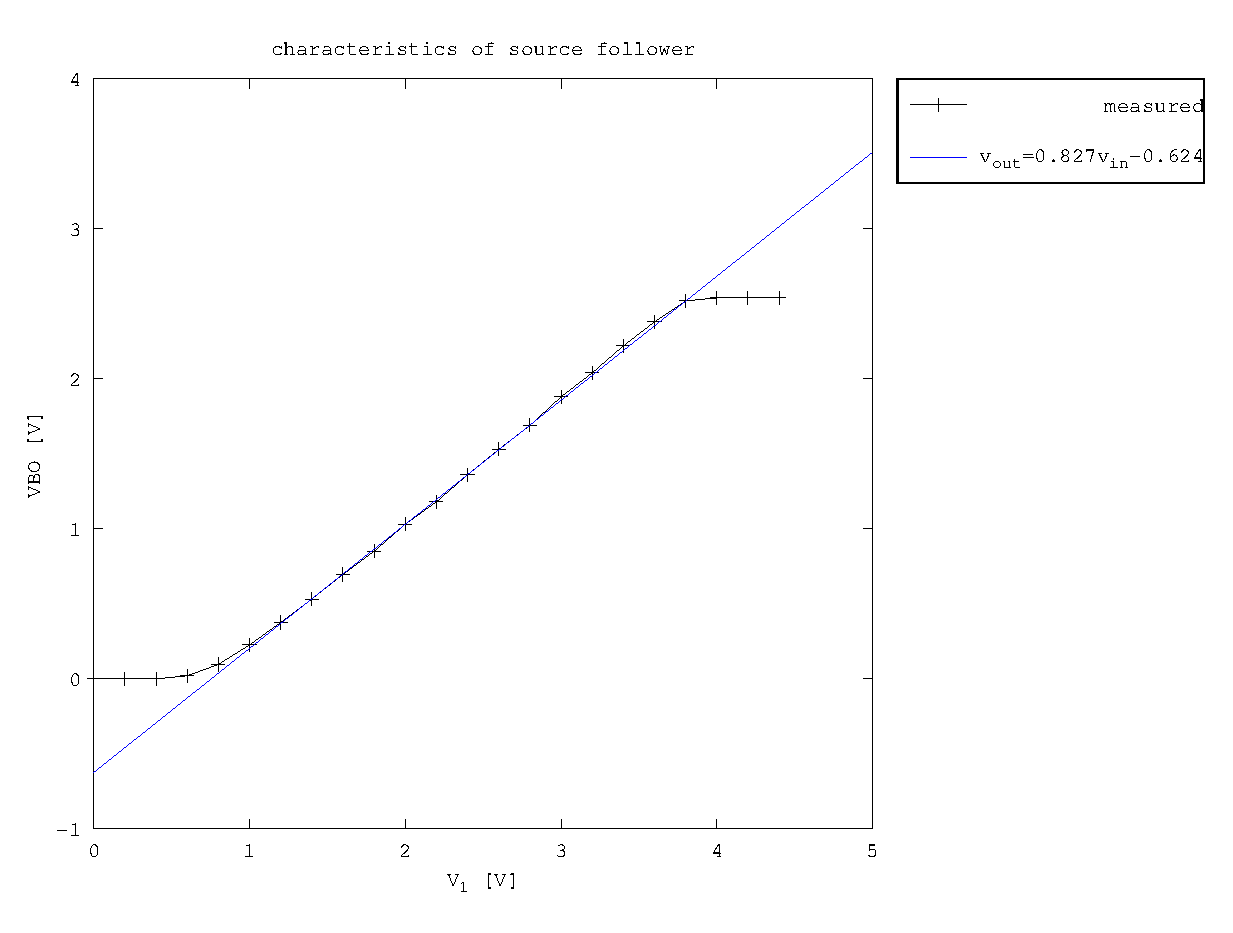
\includegraphics[width=\textwidth]{fig/source_follower.eps}
            \caption[]
                {plot of the input voltage against VBO. This plot shows the characteristics of the voltage follower}    
                \label{fig:source_follower}
        \end{figure}


\subsection{Integrator}\label{ssec:dynamic_integrator}
The measurements of the behavior of the integrator are devided into three sections. \Cref{sssec:standard_behavior} will focus on the output of the ROIC for low currents. \Cref{sssec:high_current_behavior} will do the same, but this time for currents that are a lot higher. Finally \cref{sssec:VBO_behavior} will look at the behavior of VBO, and investigate the viability of using the input follower as a secondary readout. Note that all plots are not what is directly observed at the output. All results have compensation for the behavior of the source followers.

\subsubsection{Standard behavior}\label{sssec:standard_behavior}
This test aims to address the basic relationship between input current and output voltage. \Cref{tkz:integrator_test} shows the setup used for this test. Channel 8 was used, so the end of the $20\,M\Omega$ resistor is connected to IN[8], and probes are connected to OUT[8] and VBO[8]. 

\begin{figure}[H]
\centering

\usetikzlibrary{shapes,snakes}

\newcommand*{\Vg}{Vg\\ $\color{red}4.5\,V$}
\newcommand*{\Rst}{\textbf{Rst[3]}\\ $\color{blue}reset$} 
\newcommand*{\Res}{Res\\ $\color{red}0.86\,V$}
\newcommand*{\VDD}{VDD3.3\\ $\color{red}3.3\,V$}
\newcommand*{\IN}{$\color{blue}V_{in}$}
\newcommand*{\OUT}{$\color{blue}V_{out}$}
\newcommand*{\VBO}{\color{blue}\textbf{VBO[8]} $\color{red}1.4\,V$}
\newcommand*{\gnd}{gnd\\ $\color{red}0\,V$}
\newcommand*{\C}{$\color{blue}C$}




\tikzstyle{dot} = [draw,shape=circle,fill=black, scale =.3]
\tikzstyle{l_arrow} = [draw,fill = black, regular polygon,regular polygon sides=3, rotate=-90, anchor=south, scale=.5] 
\tikzstyle{l_text} = [anchor=south west]
\tikzstyle{r_arrow} = [draw,fill = black, regular polygon,regular polygon sides=3, rotate=90, anchor=south, scale=.5] 
\tikzstyle{r_text} = [anchor=south east]
\begin{tikzpicture}[scale=1, every node/.style={scale=1}]




\draw[dashed]  (-0.5,5.5) rectangle (0.5,-2);
\node[align=center, anchor=south] at (0,5.5) {voltage\\limiter};

\draw[dashed]  (1.25,5.5) rectangle (5.25,-2);
\node[align=center, anchor=south] at (3.25,5.5) {integrator};

\draw[dashed]  (5.75,5.5) rectangle (9.25,-2);
\node[align=center, anchor=south] at (7.5,5.5) {current mirrors};

%\draw (0,0) to node[nfet]{};

%\draw (0,0) to (mos1.s);
\node(Vg)[nfet, rotate=-90] at (0,2.5) {};
\node[nfet, rotate=-90] (Reset) at (2.5,2) {};
\node[pfet] (CM_H1) at (5,3) {};
\node[nfet] (CM_L1) at (5,-1) {};
\node[nfet] (CM_H2) at (7,3) {};
\node[nfet] (CM_L2) at (7,-1) {};
\node[nfet] (CM_H3) at (9,3) {};
\node[nfet] (CM_L3) at (9,-1) {};



\draw (-1,2.5) node[anchor=east, align=center]{} to (Vg.S);
\draw (Vg.G) |- (0,4.5) node[anchor=south, align=center]{\Vg};
\draw (Vg.B) |- (1,2.5) node[dot]{} |- (CM_H1.G); %top
\draw (1,2.5) |- (1,0.5)  to [C=\C](4,0.5) -| (CM_H1.D);
\draw (1.5,0.5) node[dot]{} -| (1.5,2) |- (Reset.B);
\draw (Reset.G) to (2.5,4.5) node[anchor=south, align=center]{\Rst};
\draw (Reset.D) -| (3.5,0.5) node[dot]{};
\draw (5,0.5) node[dot]{} to (CM_L1.D);
\draw (CM_L1.G) to (4,4.5) node[anchor=south, align=center]{\Res}; 
\draw (CM_L1.S) to (CM_L2.S) to (7,-2.5) node[anchor=north, align=center]{\gnd};
\draw (CM_H1.B) |- (CM_H2.D) to (7,4.5) node[anchor=south, align=center]{\VDD};
\draw (CM_L2.G) |- (4,0) node[dot]{};
\draw (5,0.5) -| (CM_H2.G);
\draw (CM_L1.B) to (CM_L1.S);
\draw (CM_L2.B) to (CM_L2.S);
\draw (CM_H2.B) to (CM_L2.D);
\draw (CM_H3.B) to (CM_L3.D);
\draw (1,3)node[dot]{} |- (8,4) |- (CM_H3.G);
\draw (CM_H3.D) |- (CM_H2.D) node[dot]{};
\draw (CM_L3.S) |- (CM_L2.S) node[dot]{};
\draw (CM_L3.G) |- (6,0) node[dot]{};
\draw (7,1.5)node[dot]{} to (10,1.5) node[anchor=west, align=center]{\OUT};
%\draw (9,1)node[dot]{} to (10,1) node[anchor=west, align=center]{\VBO};

\draw (-2.5,2.5)node[anchor=east, align=center]{\IN} to [R=$20\,M\Omega$](-1,2.5);


\end{tikzpicture}

\caption{Schematic of ROIC channel template}
\label{tkz:integrator_test}
\end{figure}


\Cref{fig:slopes} shows the time versus voltage plot of both the VBO and OUT for a constant input voltage. The rising and falling slopes are the VBO and OUT respecively. The timescale of this plot does not allow for much inside in VBO, but it does show some interesting results for the behavior of OUT. When the reset switches, the input node immediately loses some charge. Note that the oscilloscope matches the rising edge of the reset signal to time is $0\,s$, so this drop is at $0\,s$. When the reset is switched, a capacitance is removed almost instantly. It is interesting to observe that the slope immediately after the rising edge of the reset signal is constant for all input voltages. This means that the observed slope is not limited by the reset transistor, but by the source follower that tries to keep up. This observed slope is therefore the maximum rate at which the output node can be pulled down in the current set-up. Also note that the slope gets steeper when the integrator capacitance decreases. This matches the expected behavior of $\Delta V = \frac{-q}{C}$.


\begin{figure}[h]
    \centering
    \begin{subfigure}[b]{0.475\textwidth}
            \centering
               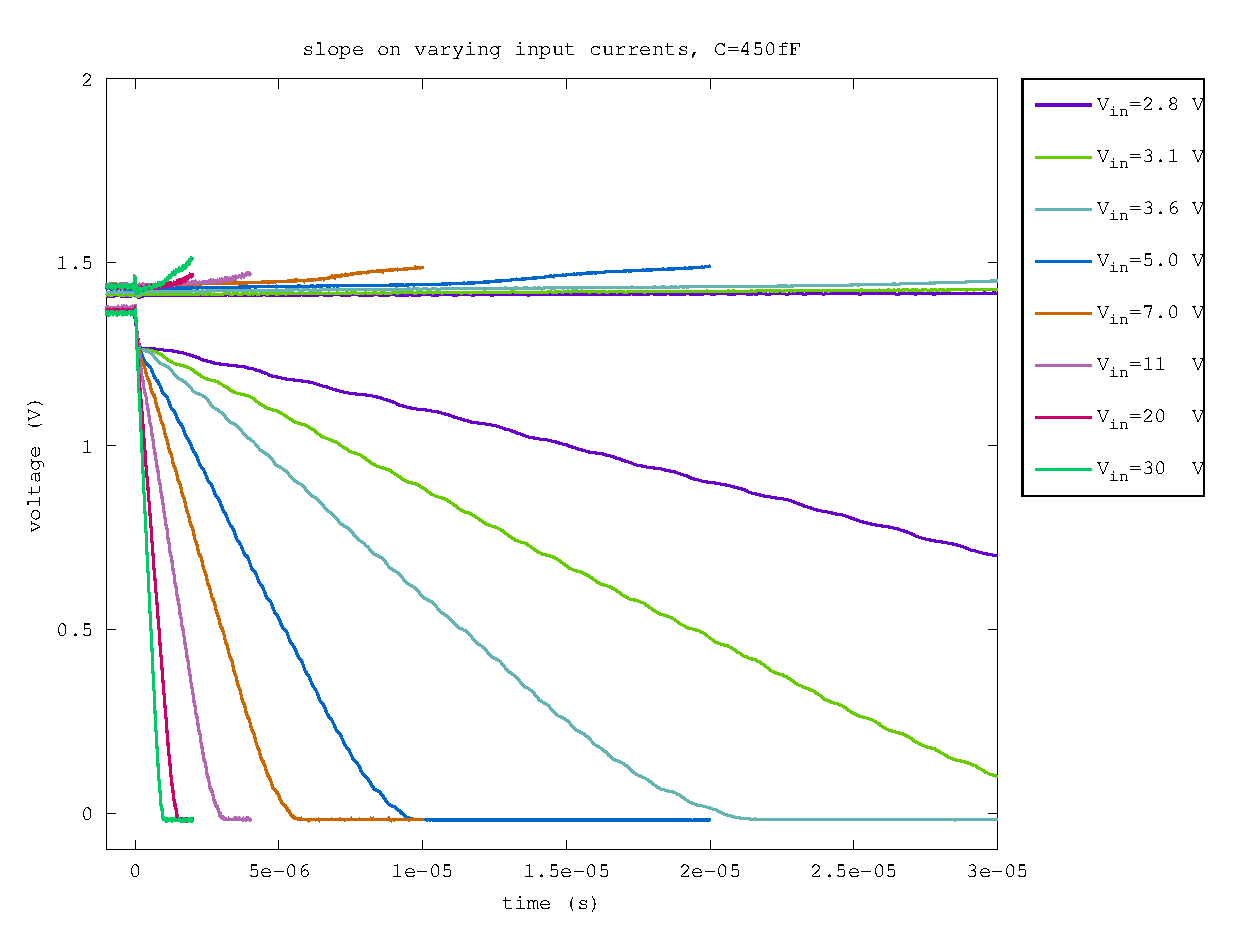
\includegraphics[width=\textwidth]{fig/slope_450fF.eps}
                    \caption[Network2]%
                        {$C=450\,fF$}    
                            \label{fig:slopes_450fF}
                        \end{subfigure}
                        \hfill
                        \begin{subfigure}[b]{0.475\textwidth}  
                                \centering 
                                    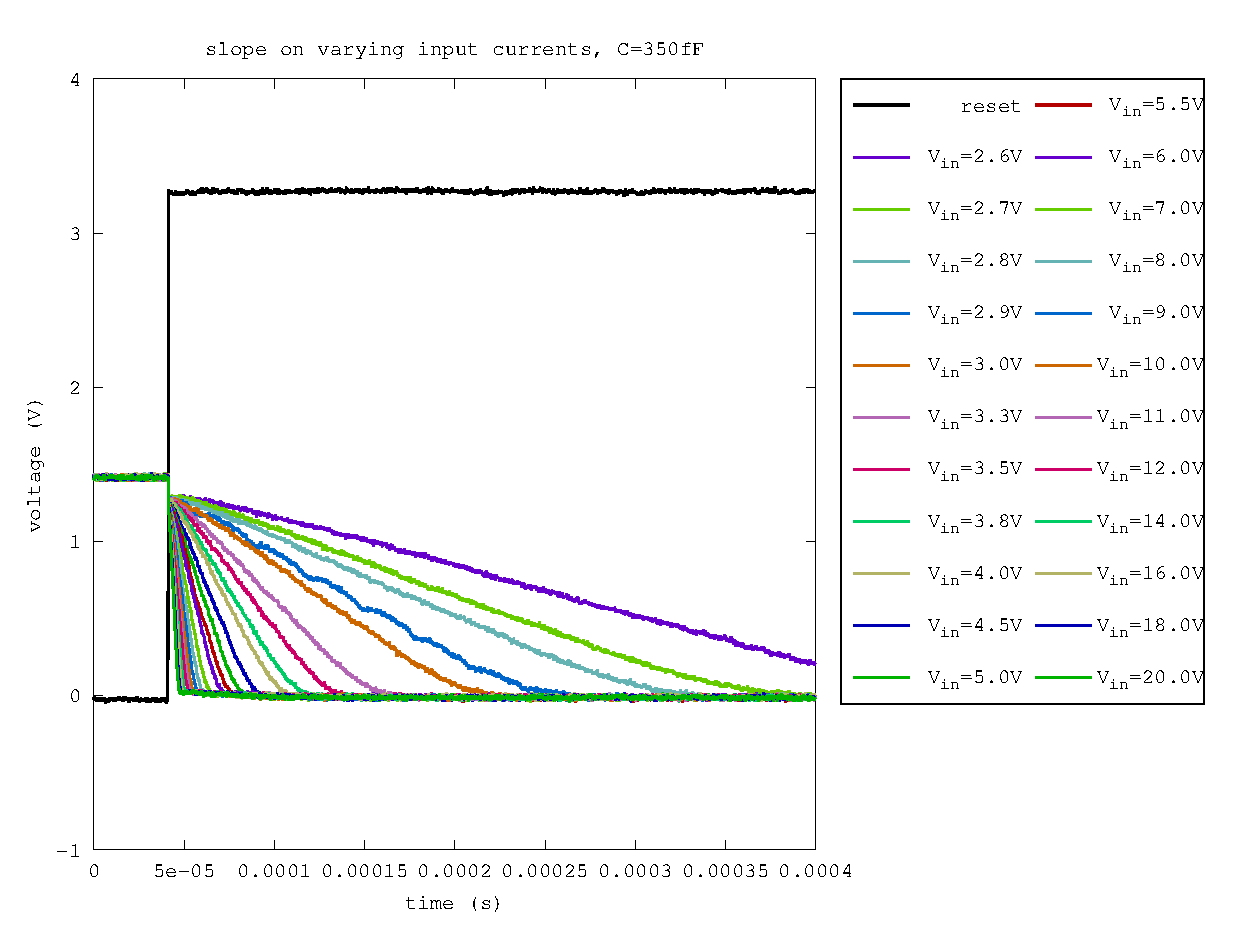
\includegraphics[width=\textwidth]{fig/slope_350fF.eps}
                                    \caption[]
                                        {$C=350\,fF$}    
                                        \label{fig:slopes_350fF}
                                \end{subfigure}
                            \vskip\baselineskip
                            \begin{subfigure}[b]{0.475\textwidth}   
                                \centering 
                                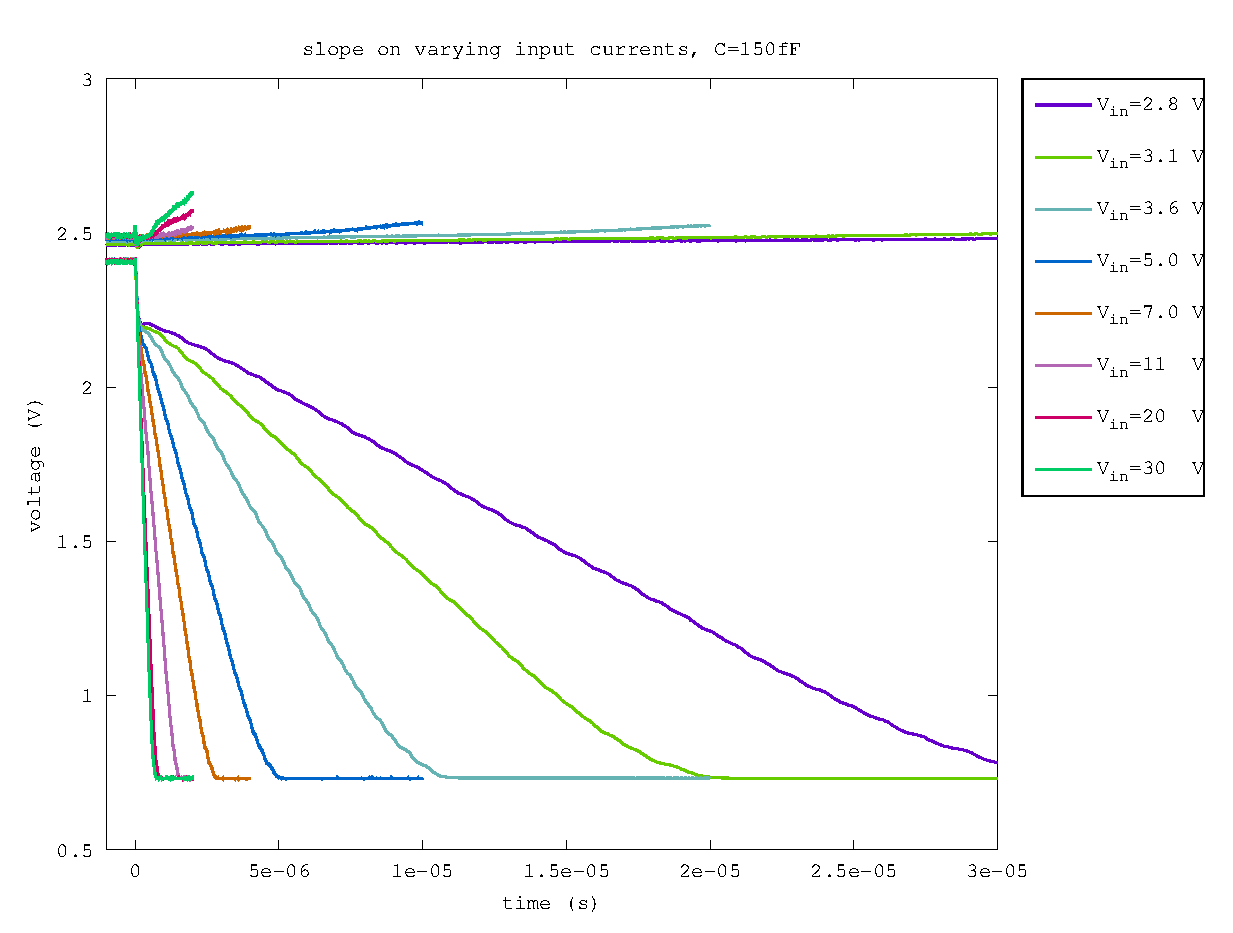
\includegraphics[width=\textwidth]{fig/slope_150fF.eps}
                                \caption[]
                                    {$C=150\,fF$}    
                                    \label{fig:slopes_150fF}
                            \end{subfigure}
                        \quad
                        \begin{subfigure}[b]{0.475\textwidth}   
                            \centering 
                            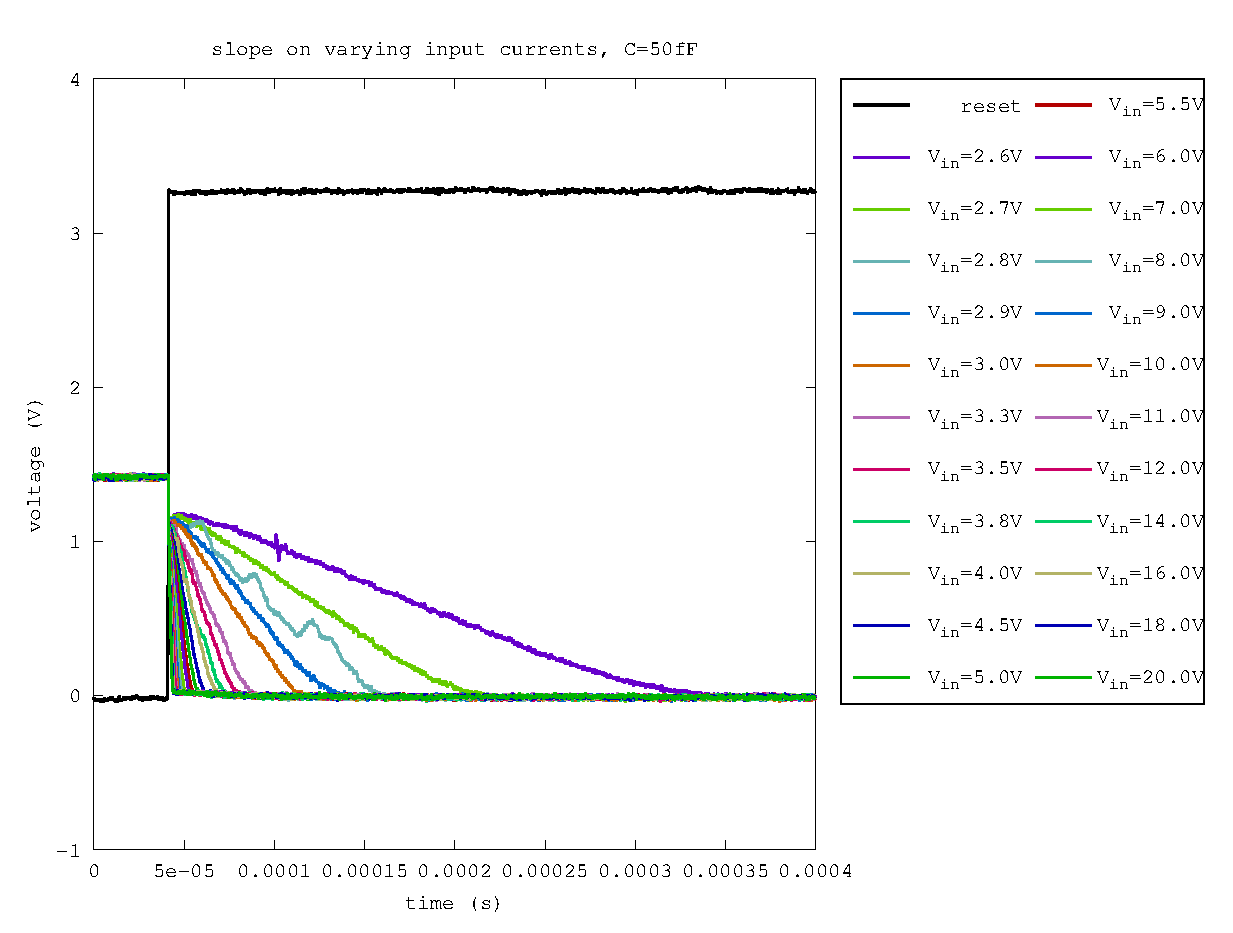
\includegraphics[width=\textwidth]{fig/slope_50fF.eps}
                            \caption[]
                                {$C=50\,fF$}    
                                \label{fig:slopes_50fF}
                        \end{subfigure}
                    \caption{Expected versus measured charge up times for different input voltages. The input voltage is connected to the input through a resistor of $20\,M\Omega$}
                \label{fig:slopes}
        \end{figure}
    
    \Cref{fig:charges} shows the same plot as \cref{fig:slopes}, but now the x axis is scaled with input current. This shows for \cref{fig:slopes_450fF} and \ref{fig:slopes_350fF} that the relationship between output voltage and charge is equal across different input voltages. For \cref{fig:slopes_150fF} and \ref{fig:slopes_50fF} however, one can see that the higher voltages lose this property. Another intersting observation is that when one looks closely at the plot, one can observe a small oscillation with a period that is constant with charge. Also the period is constant across different voltages. A hypothesis explaining this behavior has yet to be found.


    \begin{figure}[h]
    \centering
    \begin{subfigure}[b]{0.475\textwidth}
        \centering
        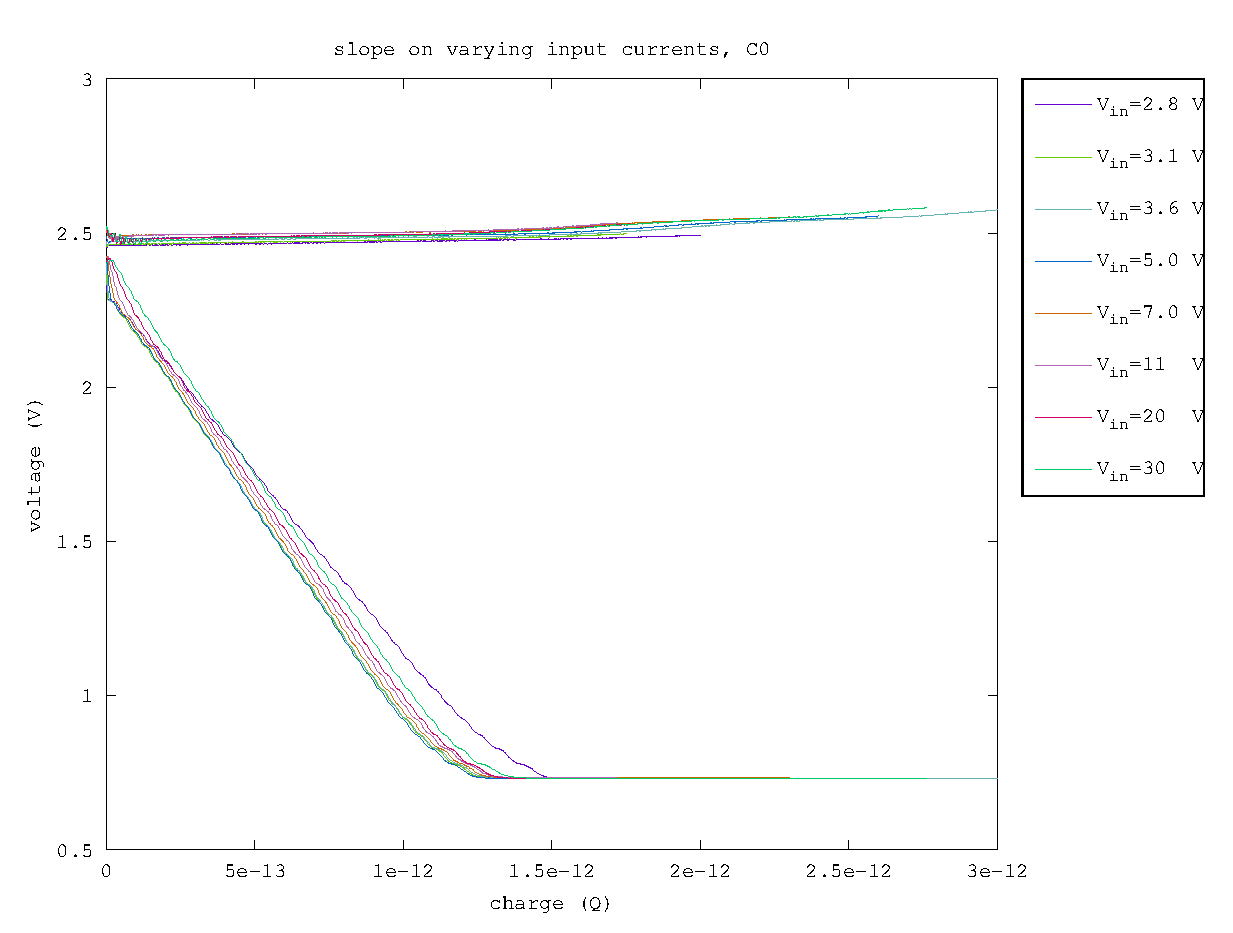
\includegraphics[width=\textwidth]{fig/charge_450fF.eps}
        \caption[Network2]%
        {$C=450\,fF$}    
        \label{fig:charges_450fF}
\end{subfigure}
\hfill
\begin{subfigure}[b]{0.475\textwidth}  
    \centering 
    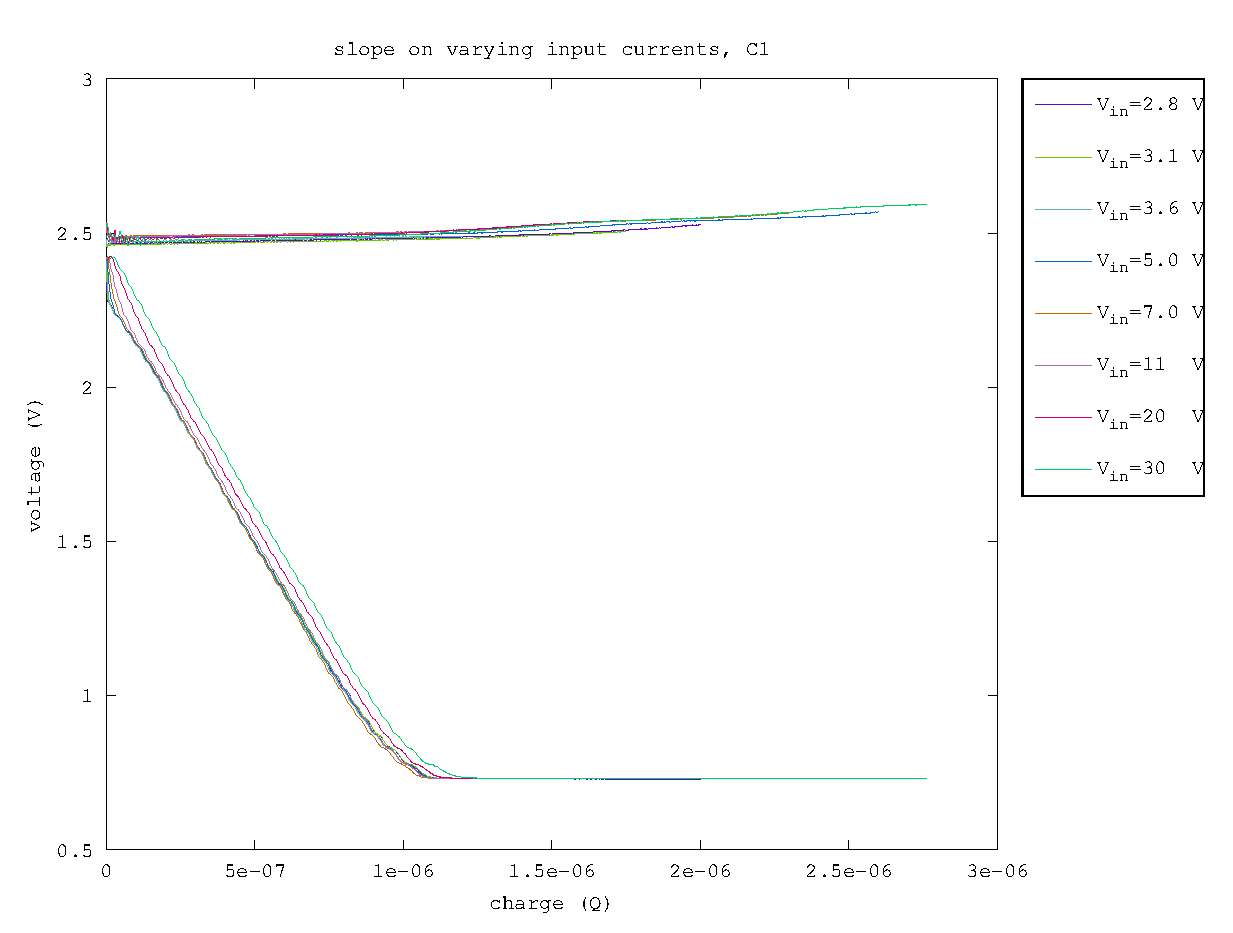
\includegraphics[width=\textwidth]{fig/charge_350fF.eps}
    \caption[]
        {$C=350\,fF$}    
        \label{fig:charges_350fF}
\end{subfigure}
\vskip\baselineskip
\begin{subfigure}[b]{0.475\textwidth}   
    \centering 
    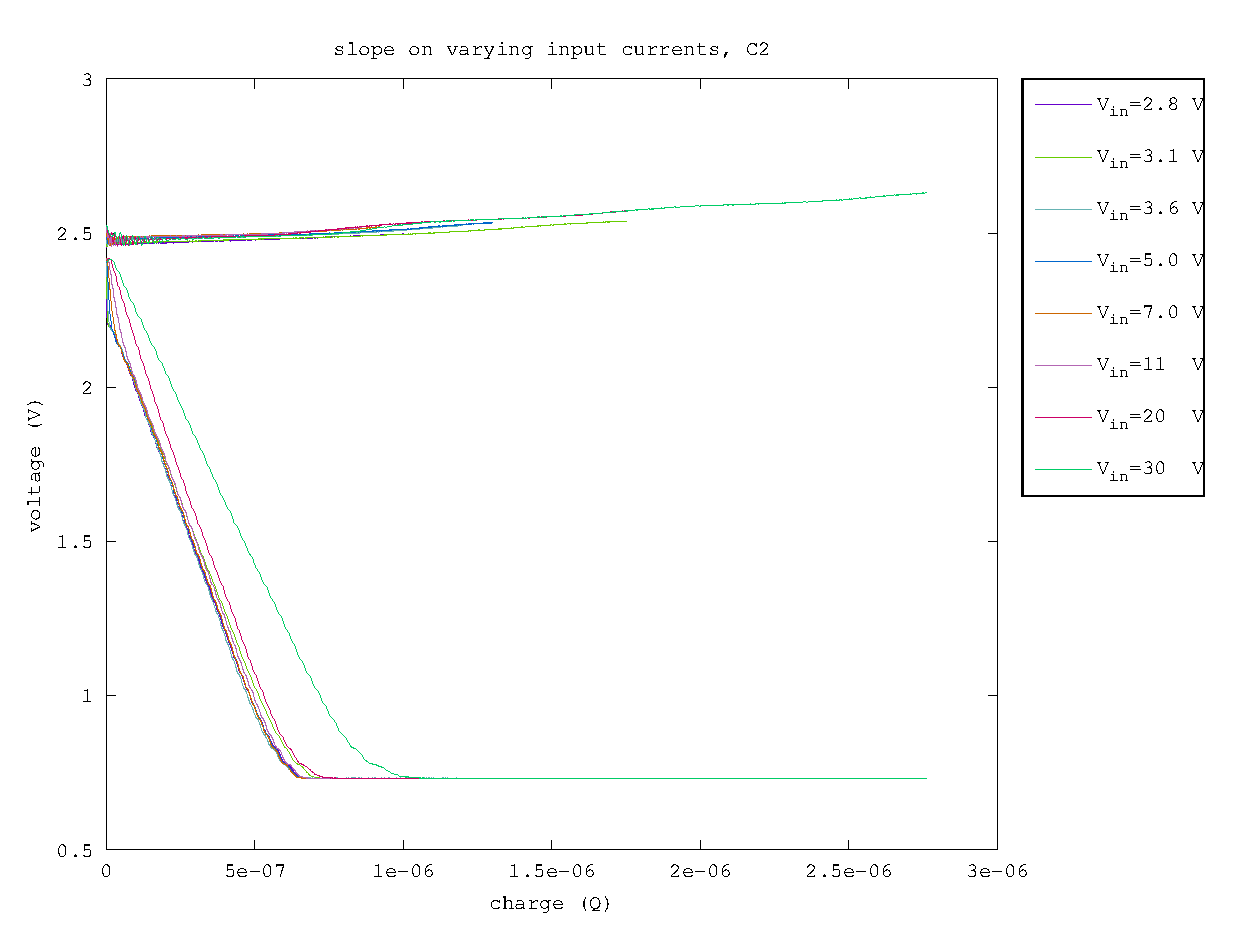
\includegraphics[width=\textwidth]{fig/charge_150fF.eps}
    \caption[]
        {$C=150\,fF$}    
        \label{fig:charges_150fF}
\end{subfigure}
\quad
\begin{subfigure}[b]{0.475\textwidth}   
    \centering 
    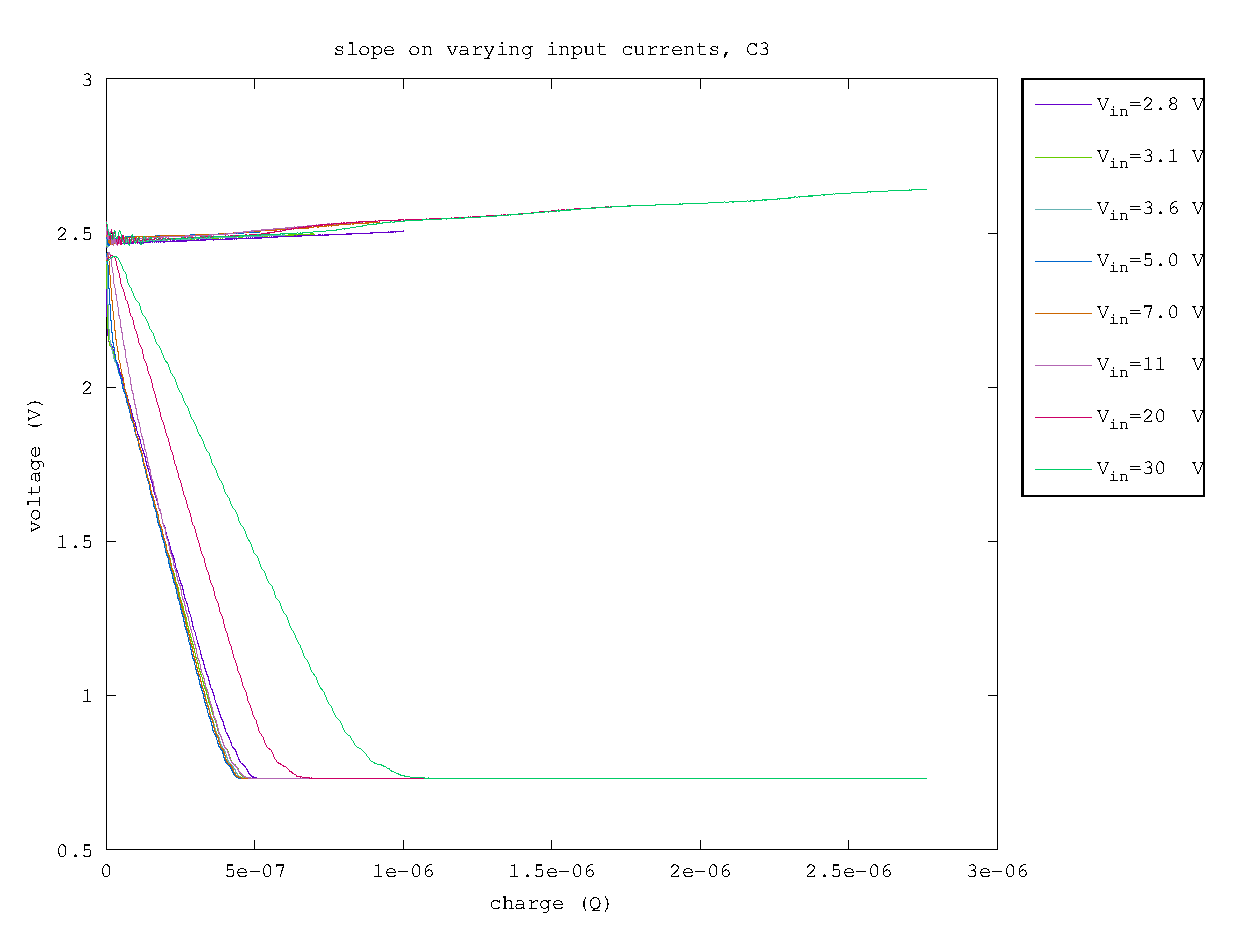
\includegraphics[width=\textwidth]{fig/charge_50fF.eps}
    \caption[]
        {$C=50\,fF$}    
        \label{fig:charges_50fF}
\end{subfigure}
\caption{This plot is showing charge versus voltage}
\label{fig:charges}
\end{figure}

\Cref{fig:d_slopes} shows the $\delta Q/\delta V$ against charge plots. Note that $\delta Q/\delta V$ is the capacitance. One can observe that while the capacitance is charging, the full value of the capacitancec can be observed, and when the capacitance is comopletely decharged, it behaves as if it is not there. One can use these plots to estimate the integration capacitance. The capitance for \cref{fig:charges_450fF}, \ref{fig:charges_350fF}, \ref{fig:charges_150fF} and \ref{fig:charges_50fF} are approxiately $450\,fF$, $350\,fF$, $220\,fF$ and $180\,fF$ respectively.


\begin{figure}[h]
\centering
\begin{subfigure}[b]{0.475\textwidth}
    \centering
    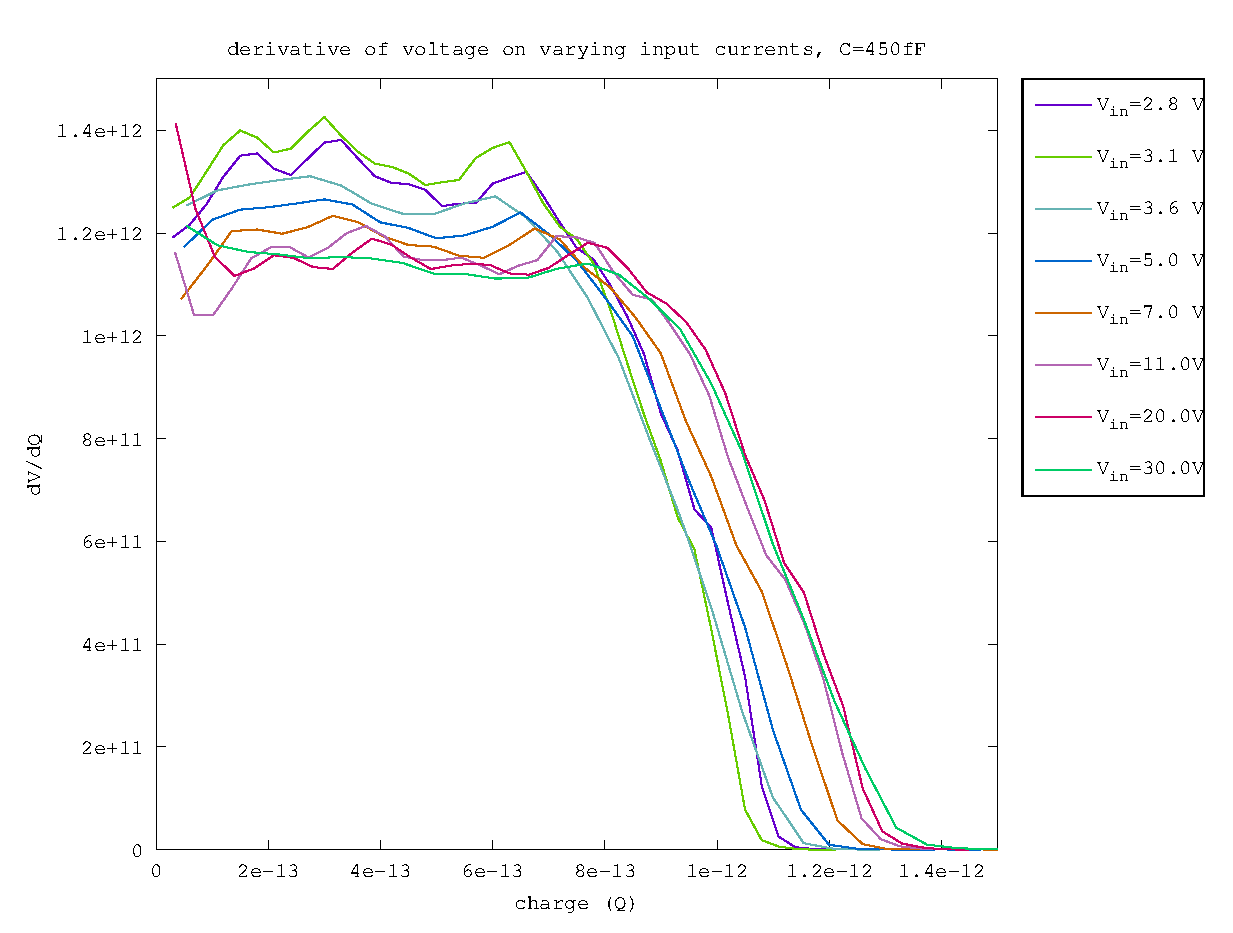
\includegraphics[width=\textwidth]{fig/d_slope_450fF.eps}
    \caption[Network2]%
    {$C=450\,fF$}    
    \label{fig:d_slopes_450fF}
\end{subfigure}
\hfill
\begin{subfigure}[b]{0.475\textwidth}  
    \centering 
    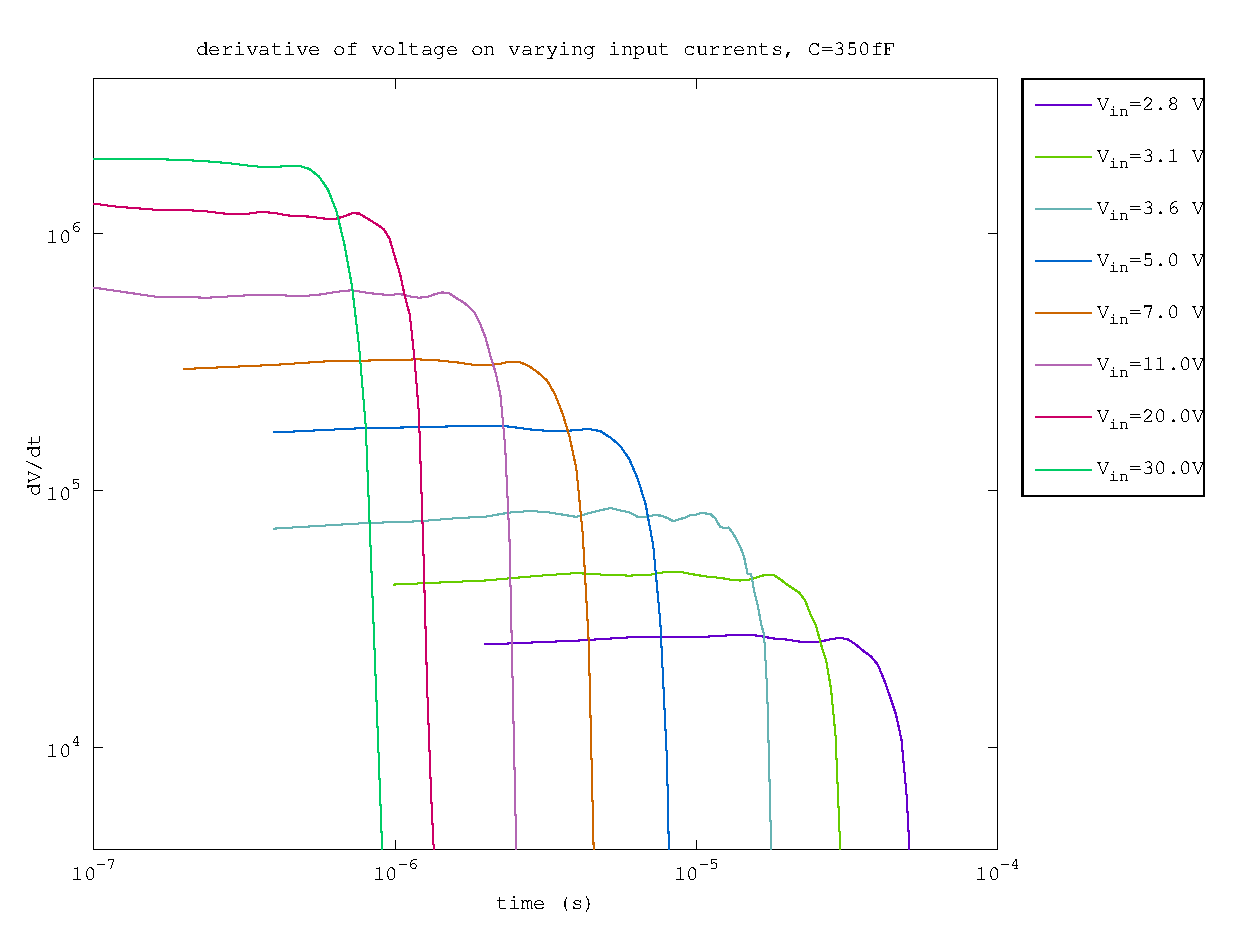
\includegraphics[width=\textwidth]{fig/d_slope_350fF.eps}
    \caption[]
        {$C=350\,fF$}    
        \label{fig:d_slopes_350fF}
\end{subfigure}
\vskip\baselineskip
\begin{subfigure}[b]{0.475\textwidth}   
    \centering 
    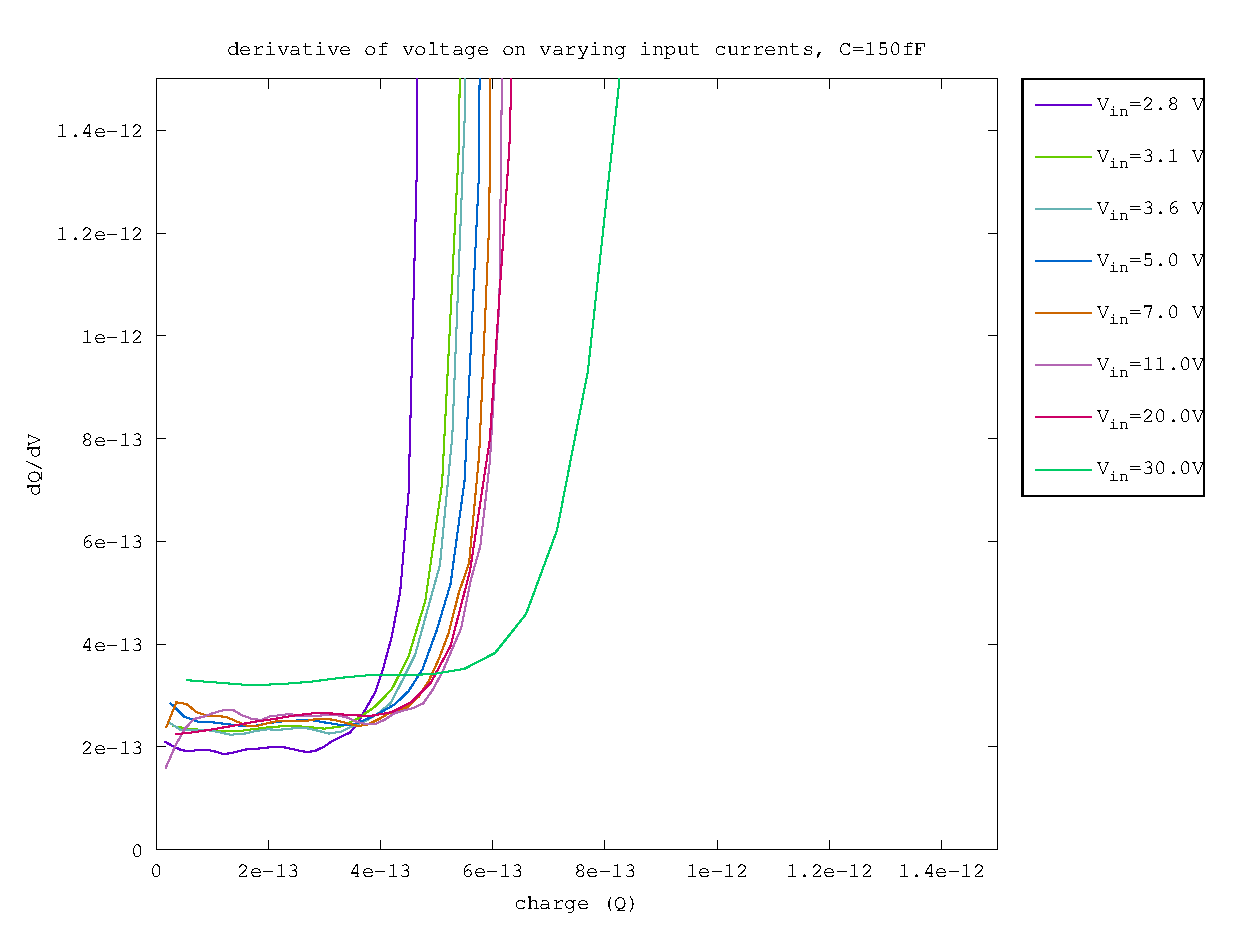
\includegraphics[width=\textwidth]{fig/d_slope_150fF.eps}
    \caption[]
        {$C=150\,fF$}    
        \label{fig:d_slopes_150fF}
\end{subfigure}
\quad
\begin{subfigure}[b]{0.475\textwidth}   
    \centering 
    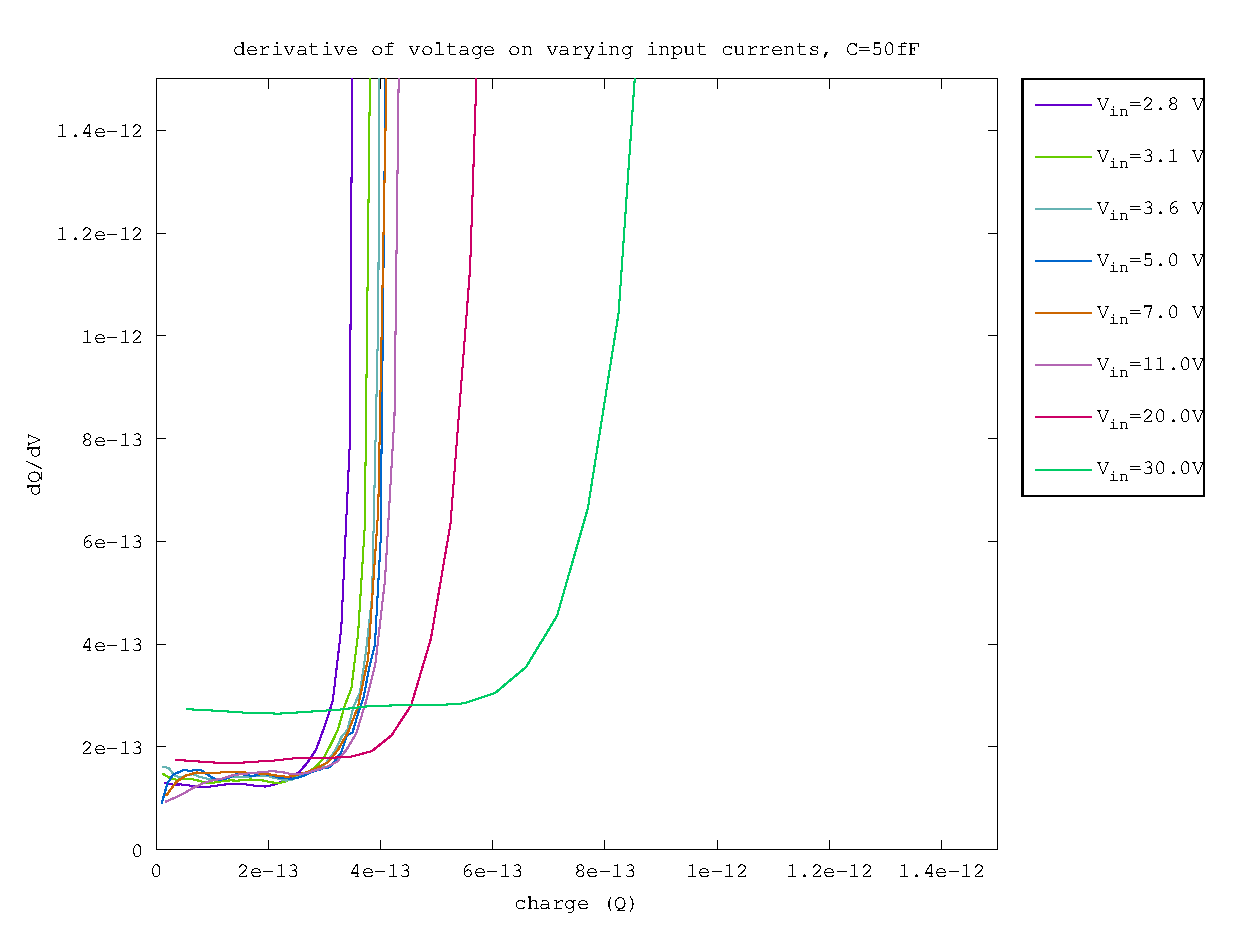
\includegraphics[width=\textwidth]{fig/d_slope_50fF.eps}
    \caption[]
        {$C=50\,fF$}    
        \label{fig:d_slopes_50fF}
\end{subfigure}
\caption{The plot shows dv/dt against time. The plot is in log scale, which allows for an easy read on the maximum slope and the time needed to discharge the integrator capacitance. }
\label{fig:d_slopes}
\end{figure}



\Cref{fig:e_vs_m} shows $\delta V / \delta t$ against input voltage for all capacitances. One can observe that all four have different slopes at first, but there appears to be a trend that they all converge to a value of $\delta V/\delta t \approx 3.2\cdot10^6$.


\begin{figure}[h]
    \centering
    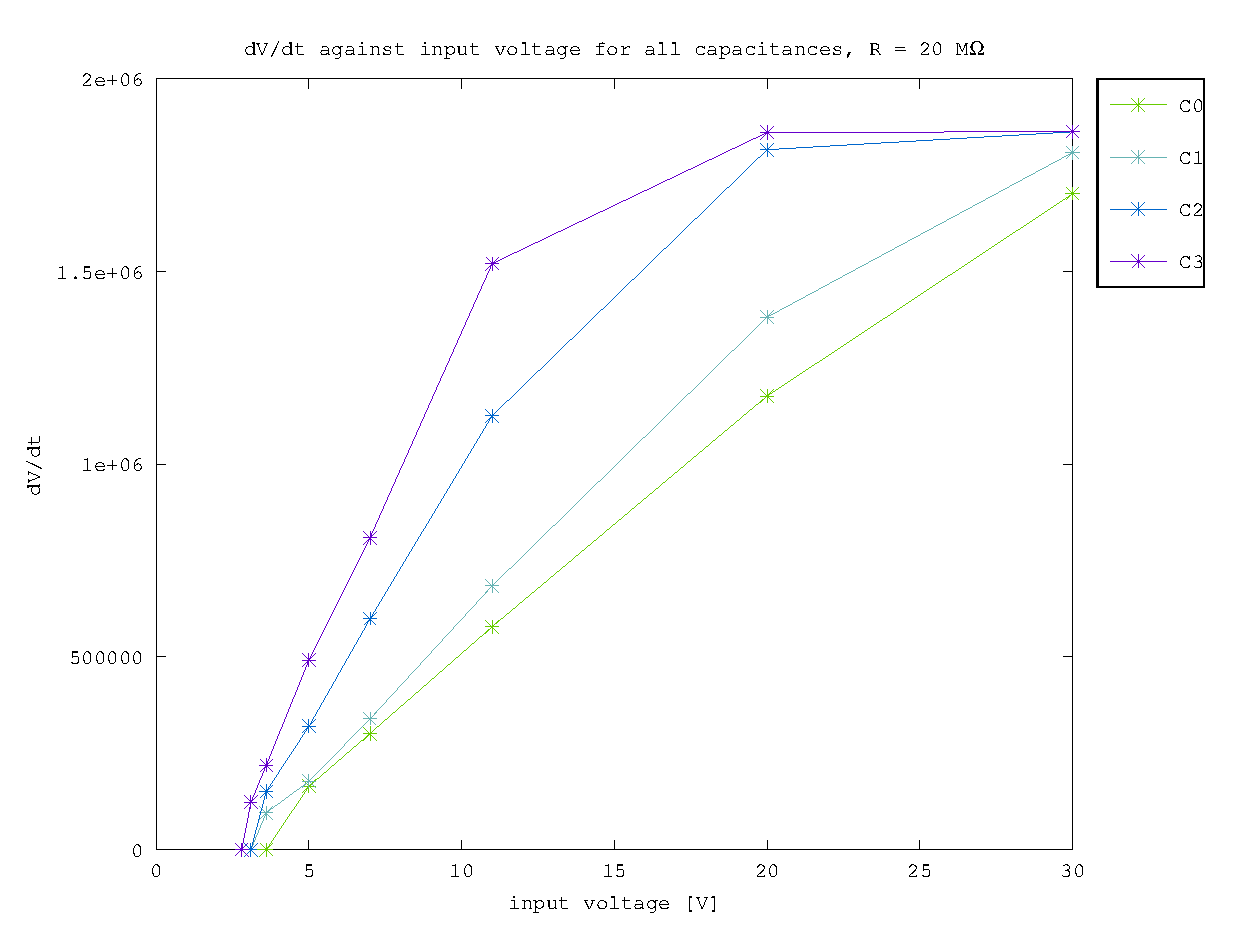
\includegraphics[width=\textwidth]{fig/vin_vs_time_sat.eps}
    \caption[]
        {dV/dt against input voltage for all four capacitances. The x indicate the measurements.}    
        \label{fig:e_vs_m}
\end{figure}

\clearpage
\subsubsection{High current behavior}\label{sssec:high_current_behavior}
In this section the $20\,M\Omega$ input resistor is replaecd with a $4\,M\Omega$ resistor. The main goal is to observe the ROIC for very large currents.


\Cref{fig:bre_slopes} shows the same plot as \cref{fig:slopes}, but this time with larger currents. Where a minimum slope could be observed at \cref{fig:slopes}, it is more prevalent here. This also shows more information about the behavior of VBO. For small voltages the VBO does not increase, but as the voltages get larger, one can observe that the voltages of VBO start rising when the OUT is done with decharging. It is also interesting to note that VBO seems to be not affected by the minimum slope at OUT. This gives rise to the hypothesis that the OUT is limited by the source follower. 

\begin{figure}[h]
    \centering
    \begin{subfigure}[b]{0.475\textwidth}
        \centering
        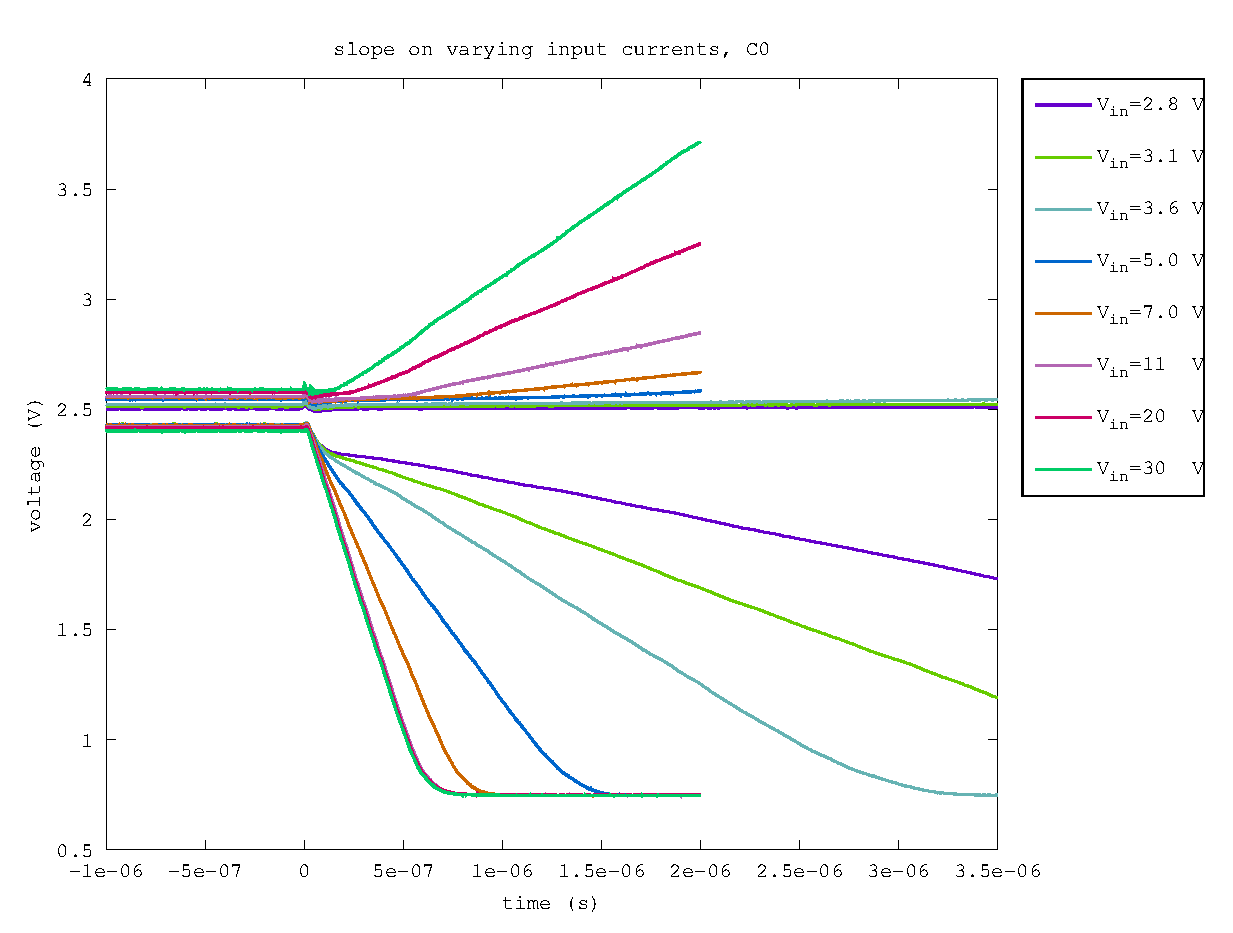
\includegraphics[width=\textwidth]{fig/bre_slope_450fF.eps}
        \caption[Network2]%
        {$C=450\,fF$}    
        \label{fig:bre_slopes_450fF}
    \end{subfigure}
    \hfill
    \begin{subfigure}[b]{0.475\textwidth}  
        \centering 
        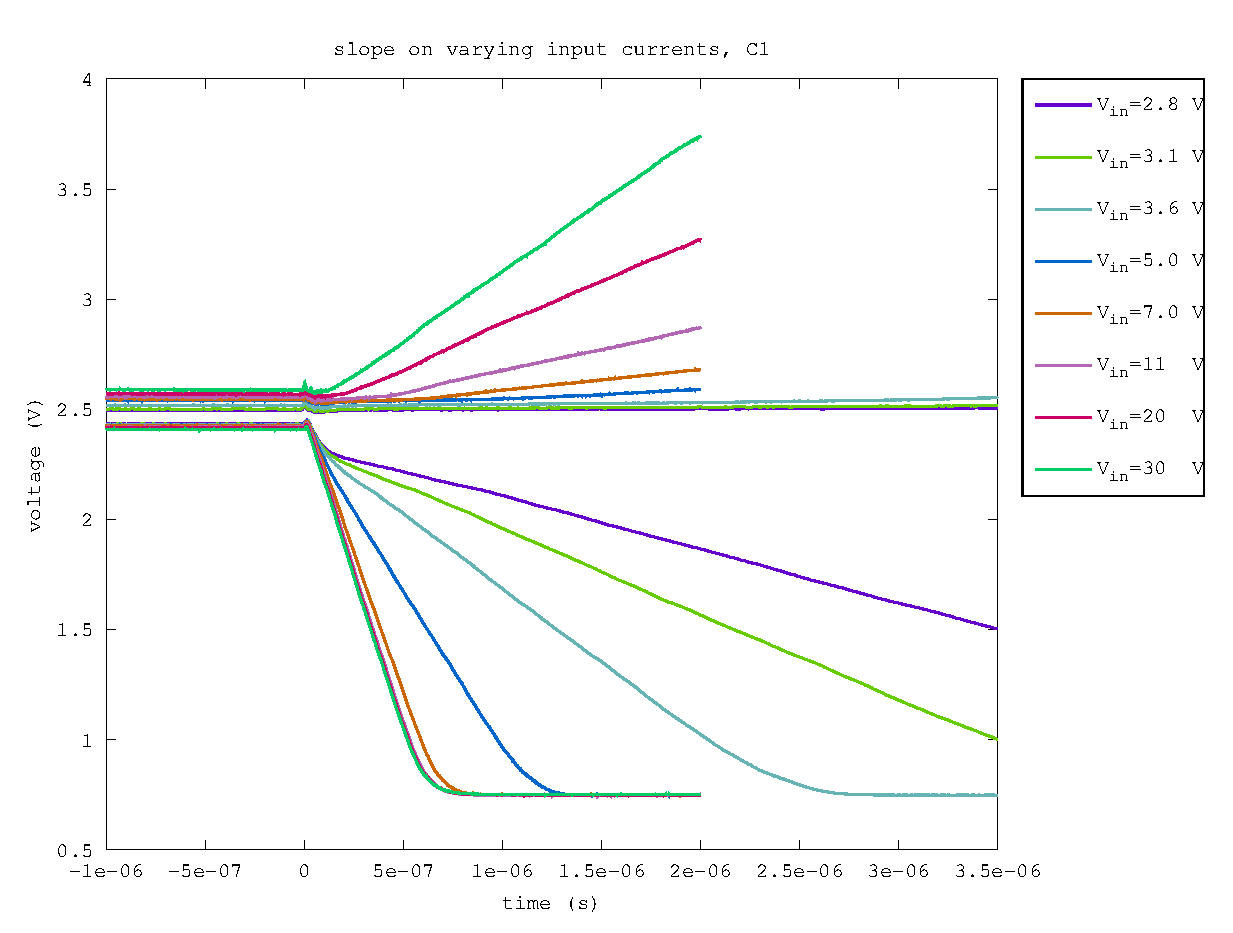
\includegraphics[width=\textwidth]{fig/bre_slope_350fF.eps}
        \caption{$C=350\,fF$}    
        \label{fig:bre_slopes_350fF}
    \end{subfigure}
    \vskip\baselineskip
    \begin{subfigure}[b]{0.475\textwidth}   
        \centering 
        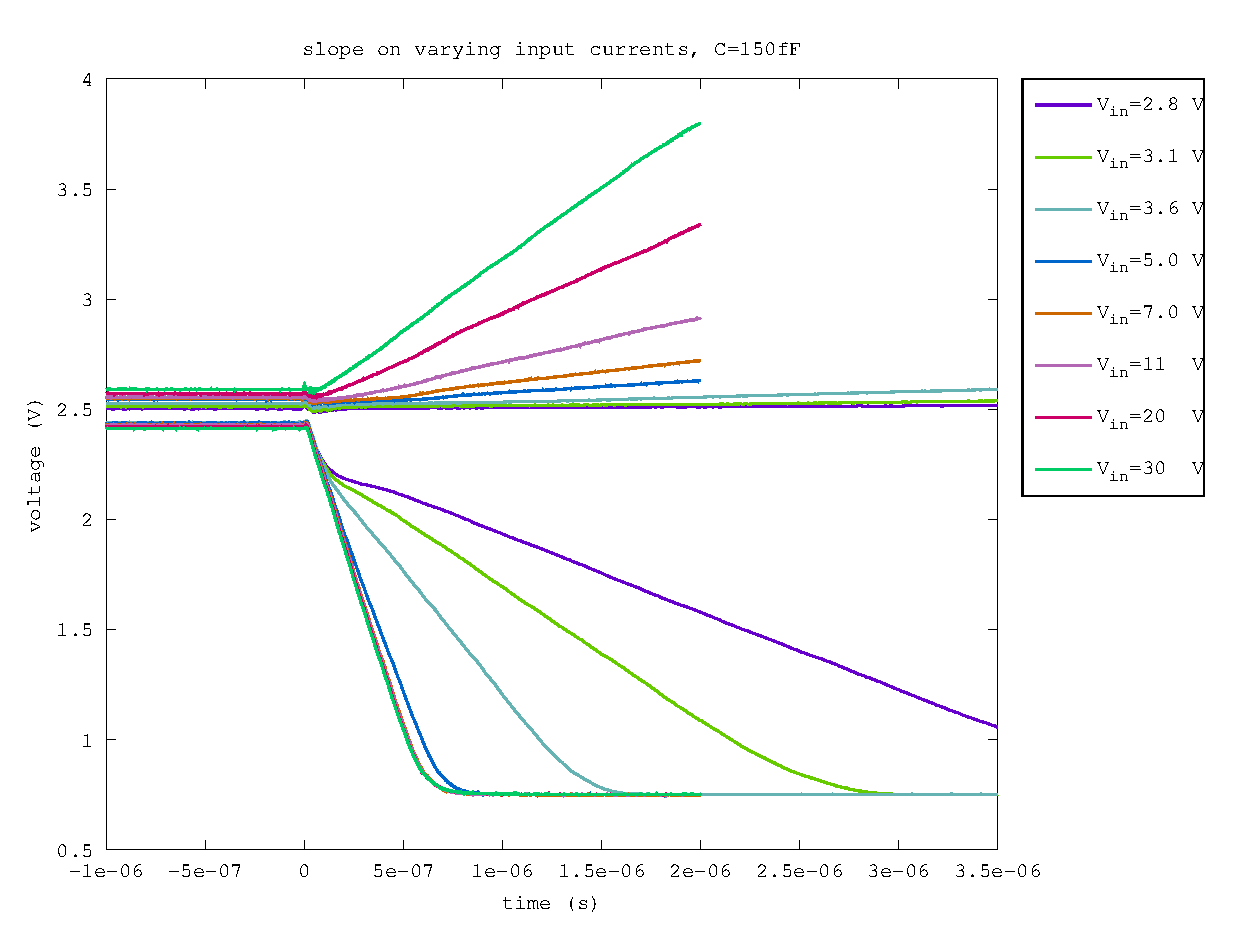
\includegraphics[width=\textwidth]{fig/bre_slope_150fF.eps}
        \caption{$C=150\,fF$}    
        \label{fig:bre_slopes_150fF}
    \end{subfigure}
    \quad
    \begin{subfigure}[b]{0.475\textwidth}   
        \centering 
        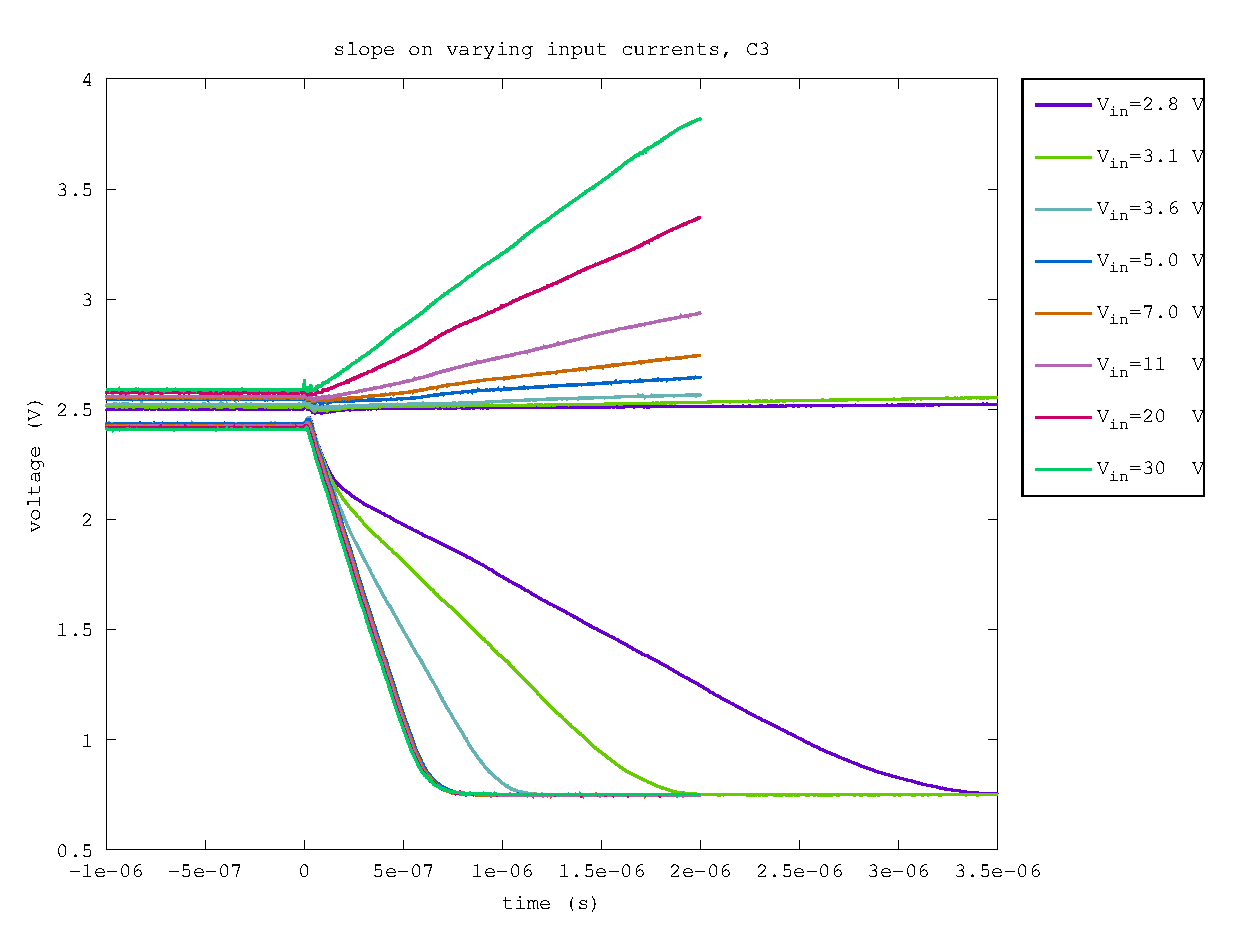
\includegraphics[width=\textwidth]{fig/bre_slope_50fF.eps}
        \caption{$C=50\,fF$}    
        \label{fig:bre_slopes_50fF}
    \end{subfigure}
    \caption{Expected versus measured charge up times for different input voltages. The input voltage is connected to the input through a resistor of $4\,M\Omega$}
    \label{fig:bre_slopes}
\end{figure}

\Cref{fig:bre_charges} shows a similar plot as in \cref{fig:charges} but with higher currents. In \cref{fig:charges} one could observe that all currents fitted to the same line, but deviated at higher currents. This effect is also observed here, but in a stronger form. Which is to be expected.

\begin{figure}[h]
    \centering
    \begin{subfigure}[b]{0.475\textwidth}
        \centering
        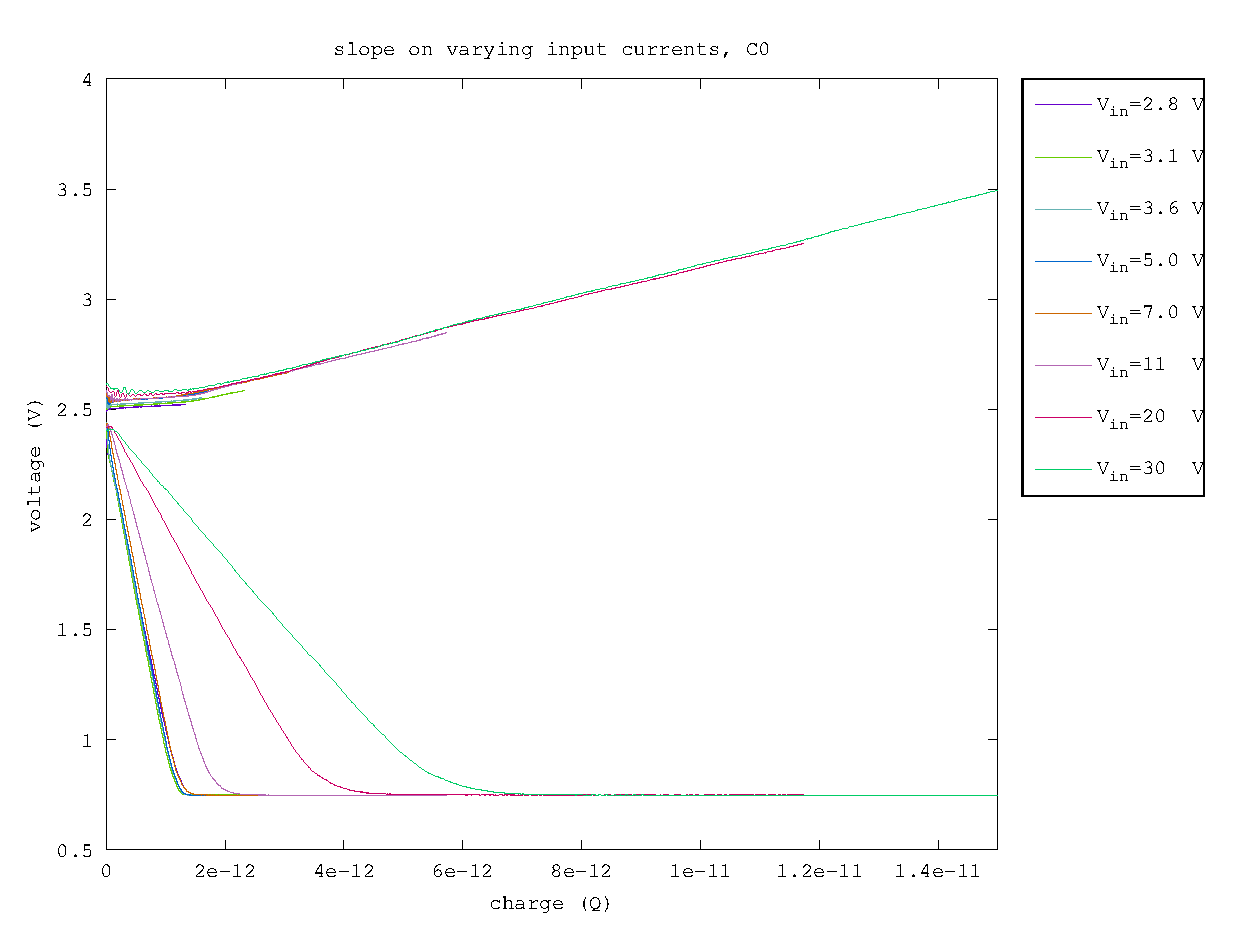
\includegraphics[width=\textwidth]{fig/bre_charge_450fF.eps}
        \caption[Network2]%
        {$C=450\,fF$}    
        \label{fig:bre_charges_450fF}
    \end{subfigure}
    \hfill
    \begin{subfigure}[b]{0.475\textwidth}  
        \centering 
        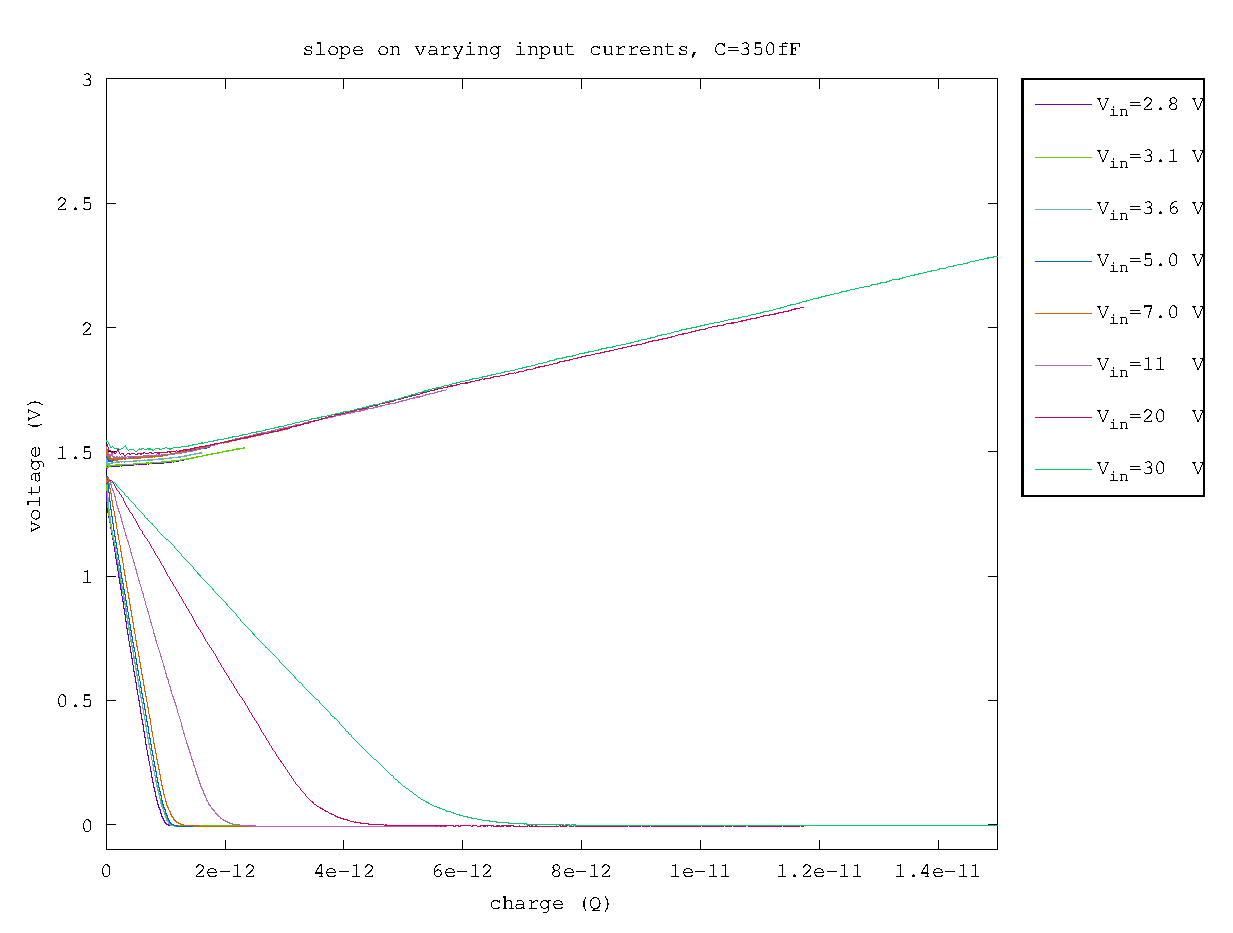
\includegraphics[width=\textwidth]{fig/bre_charge_350fF.eps}
        \caption{$C=350\,fF$}    
        \label{fig:bre_charges_350fF}
    \end{subfigure}
    \vskip\baselineskip
    \begin{subfigure}[b]{0.475\textwidth}   
        \centering 
        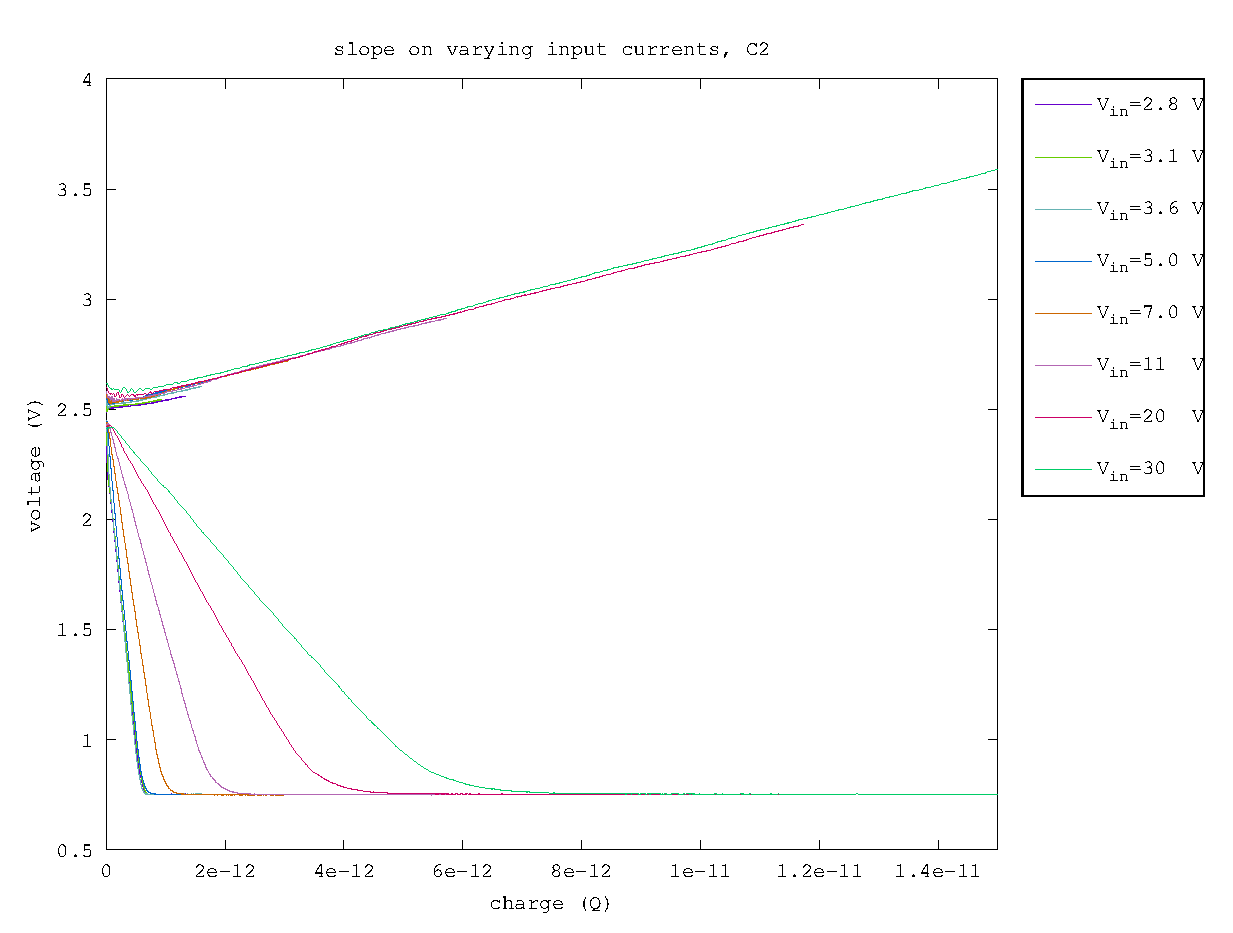
\includegraphics[width=\textwidth]{fig/bre_charge_150fF.eps}
        \caption{$C=150\,fF$}    
        \label{fig:bre_charges_150fF}
    \end{subfigure}
    \quad
    \begin{subfigure}[b]{0.475\textwidth}   
        \centering 
        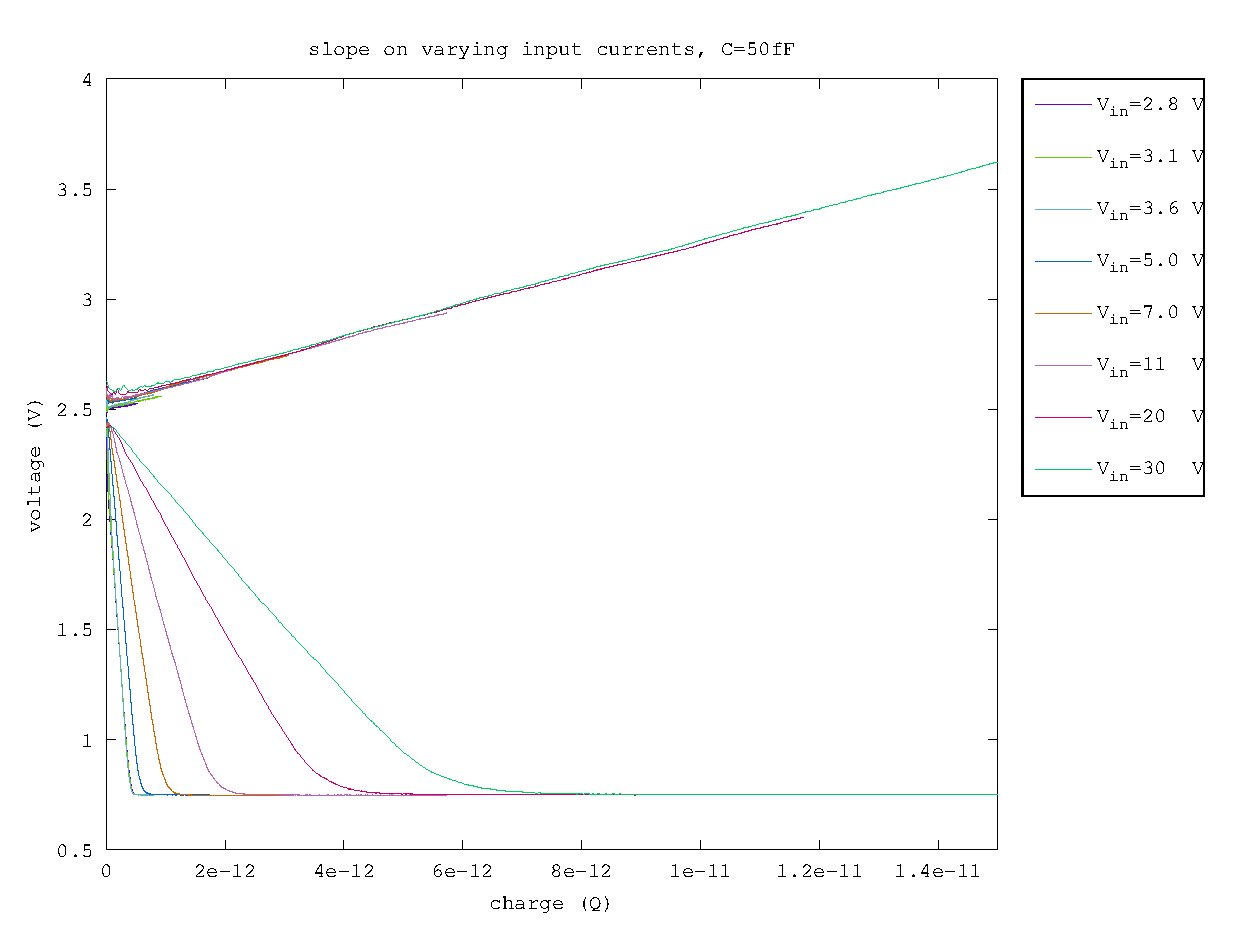
\includegraphics[width=\textwidth]{fig/bre_charge_50fF.eps}
        \caption {$C=50\,fF$}    
        \label{fig:bre_charges_50fF}
    \end{subfigure}
    \caption{This plot is showing charge versus voltage}
    \label{fig:bre_charges}
\end{figure}

\Cref{fig:bre_d_slopes} shows a plot of $\delta V/\delta Q$ against charge. Note that the behavior for the low voltages differ across the different capacitances, but that the high voltages are not affected by a change in capacitance. This observation agrees with the hypothesis that the output is not limited by the input current, but by the speed of the source follower at the output.

\begin{figure}[h]
    \centering
    \begin{subfigure}[b]{0.475\textwidth}
        \centering
        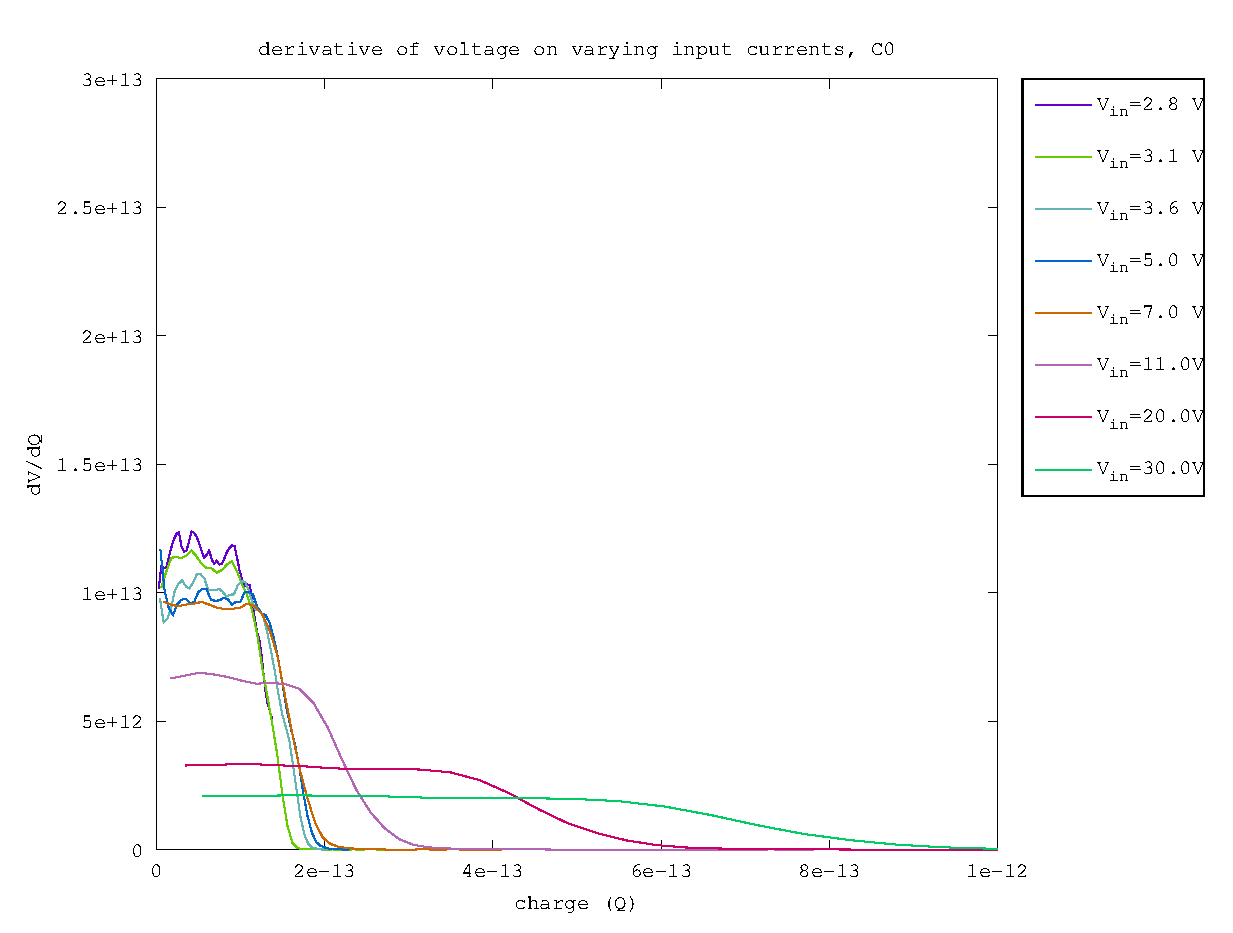
\includegraphics[width=\textwidth]{fig/bre_d_slope_450fF.eps}
        \caption[Network2]%
        {$C=450\,fF$}    
        \label{fig:bre_d_slopes_450fF}
    \end{subfigure}
    \hfill
    \begin{subfigure}[b]{0.475\textwidth}  
        \centering 
        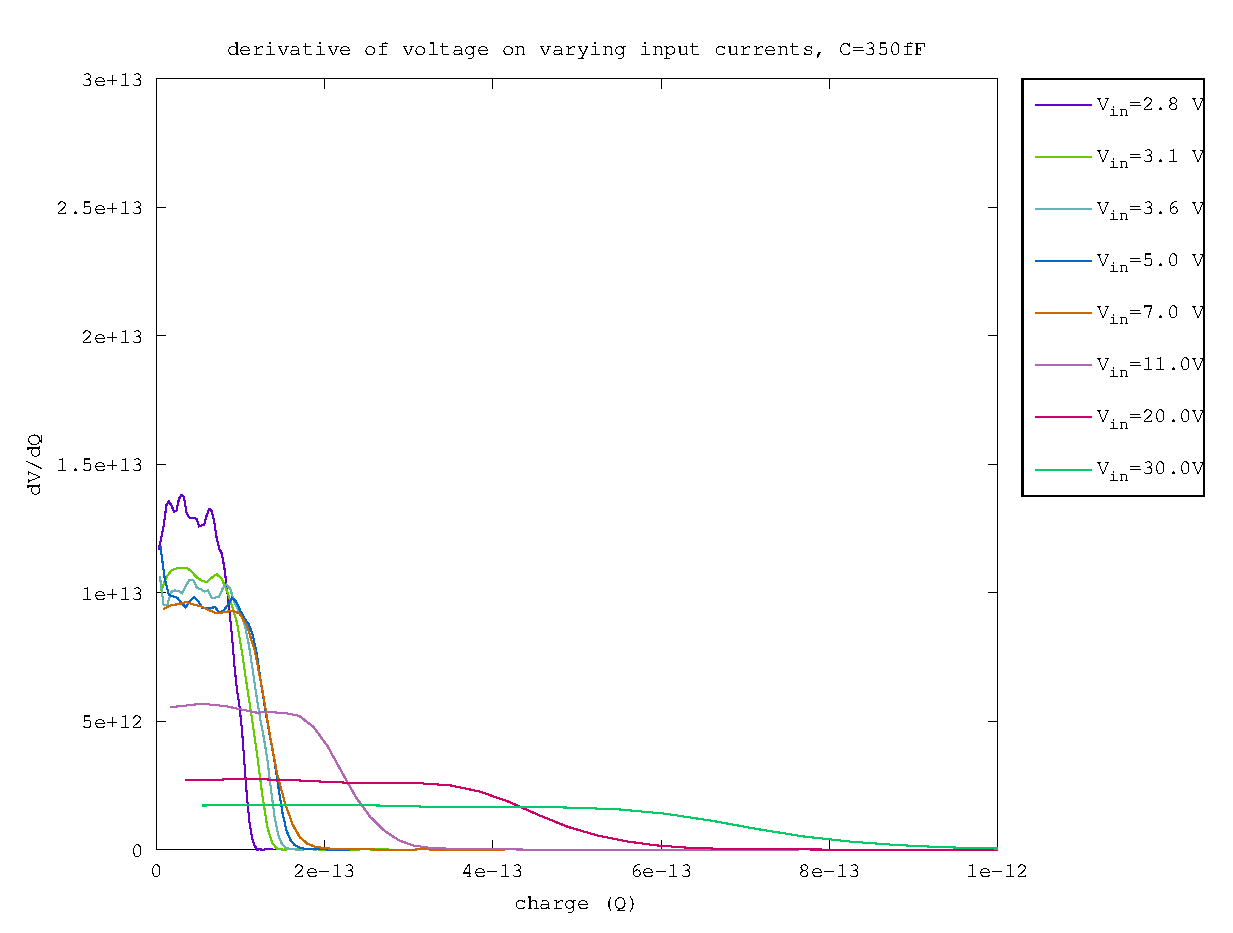
\includegraphics[width=\textwidth]{fig/bre_d_slope_350fF.eps}
        \caption {$C=350\,fF$}    
        \label{fig:bre_d_slopes_350fF}
    \end{subfigure}
    \vskip\baselineskip
    \begin{subfigure}[b]{0.475\textwidth}   
        \centering 
        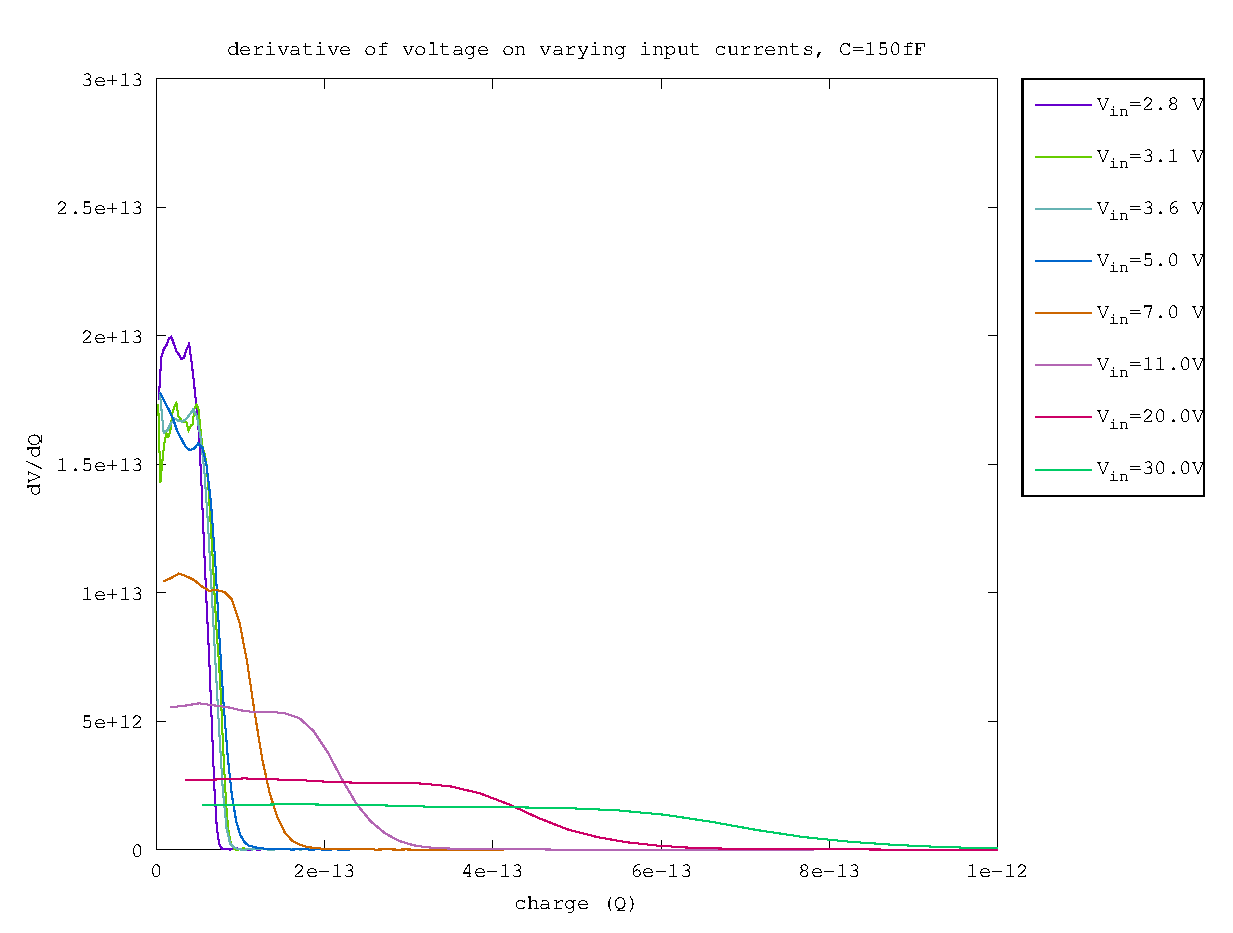
\includegraphics[width=\textwidth]{fig/bre_d_slope_150fF.eps}
        \caption {$C=150\,fF$}    
        \label{fig:bre_d_slopes_150fF}
    \end{subfigure}
    \quad
    \begin{subfigure}[b]{0.475\textwidth}   
        \centering 
        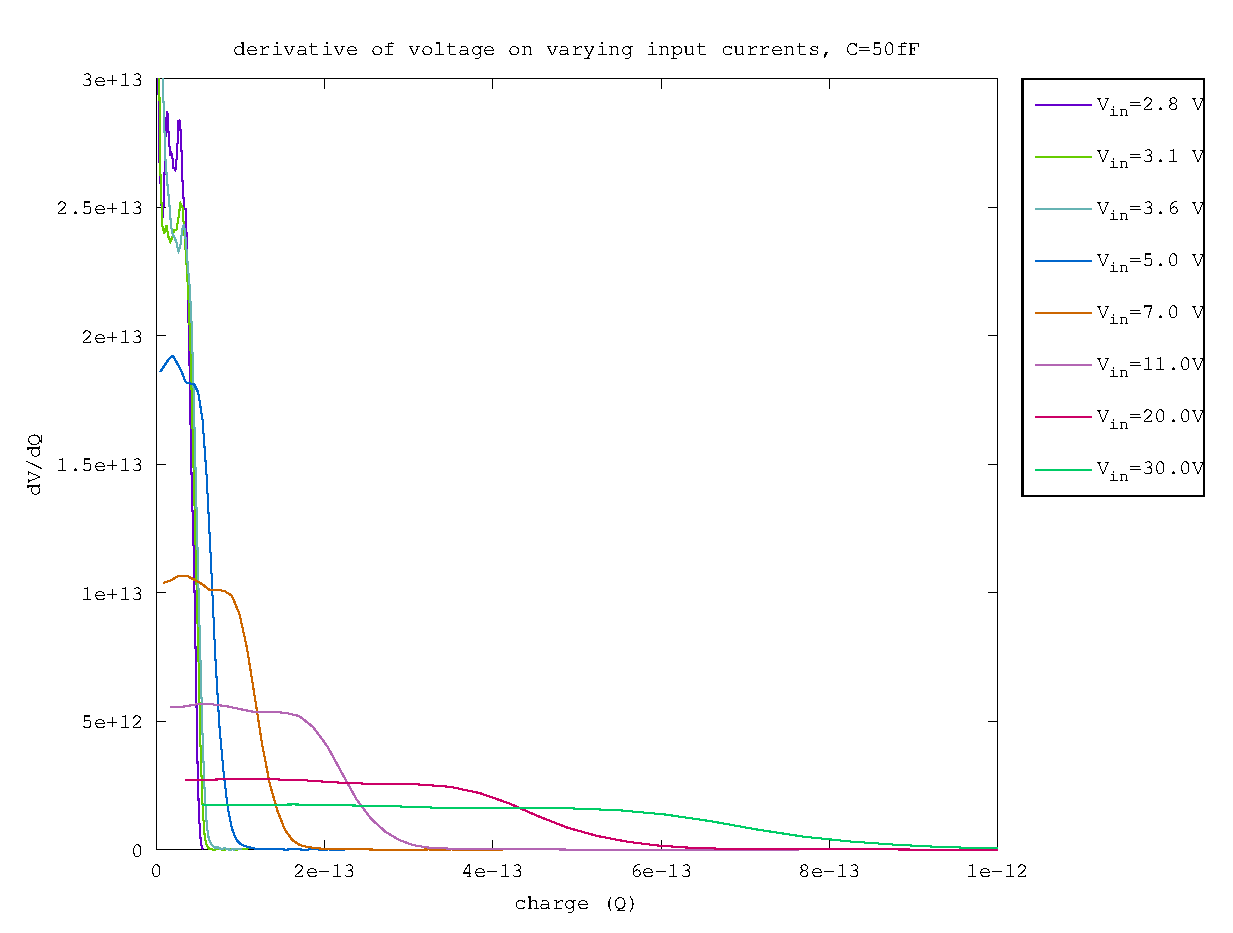
\includegraphics[width=\textwidth]{fig/bre_d_slope_50fF.eps}
        \caption{$C=50\,fF$}    
        \label{fig:bre_d_slopes_50fF}
    \end{subfigure}
    \caption{The plot shows dv/dt against time. The plot is in log scale, which allows for an easy read on the maximum slope and the time needed to discharge the integrator capacitance. }
    \label{fig:bre_d_slopes}
\end{figure}

\Cref{fig:bre_e_vs_m} shows the same plot as \cref{fig:e_vs_m}, but with higher current. This plot clearly shows that all four capacitance configurations saturate at a $\delta V\delta t \approx 3.1\,V$. This cannot be a limit applied to the input, because the capacitances are different. Therefore the output is limiting this, conform previous observations.

\begin{figure}[h]
    \centering
    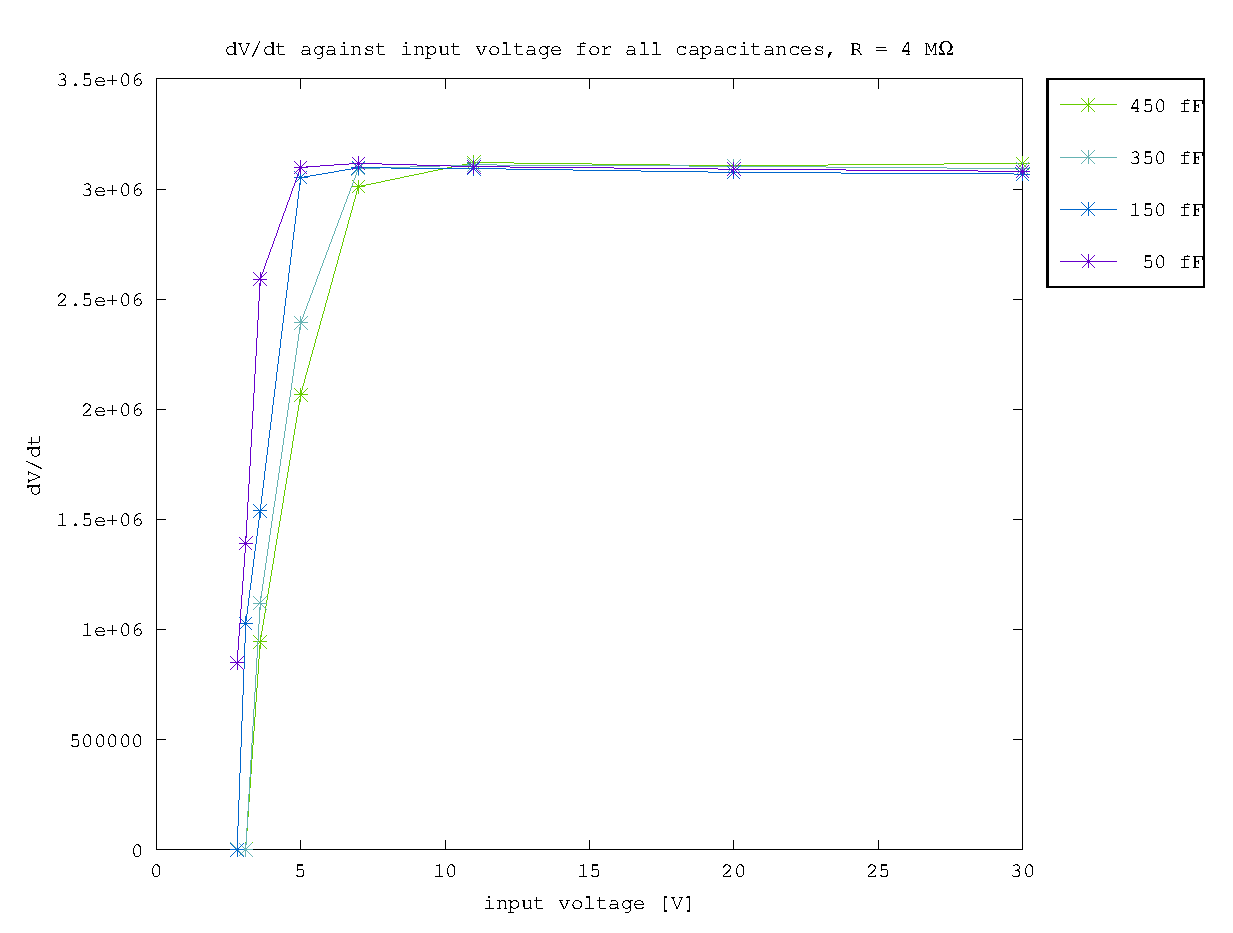
\includegraphics[width=\textwidth]{fig/bre_vin_vs_time_sat.eps}
    \caption {dV/dt against input voltage for all four capacitances. The x indicate the measurements.}    
    \label{fig:bre_e_vs_m}
\end{figure}

\clearpage
\subsubsection{VBO behavior}\label{sssec:VBO_behavior}


\subsection{Voltage limiter}\label{ssec:dynamic_voltage_limiter}


